\chapter{ Le vademecum du Modèle Standard }
\renewcommand\chapterillustration{SM/sm2}
\ThisULCornerWallPaper{1}{\chapterillustration}
\minitoc
\lettrine[lines=4, slope=-0.5em]{D}{ans} ce chapitre, un bref historique de la Physique des particules est donné ainsi qu'un résumé et une description de la théorie la plus aboutie dans ce domaine, appelée le Modèle Standard (MS). Il sera également discuté des faiblesses et limites de cette théorie ainsi que de ses éventuelles extensions.
\vspace*{-0.4cm}
\section{Un bref historique}
\vspace*{-0.4cm}
\marginpar
{
\centering
%\begin{center}
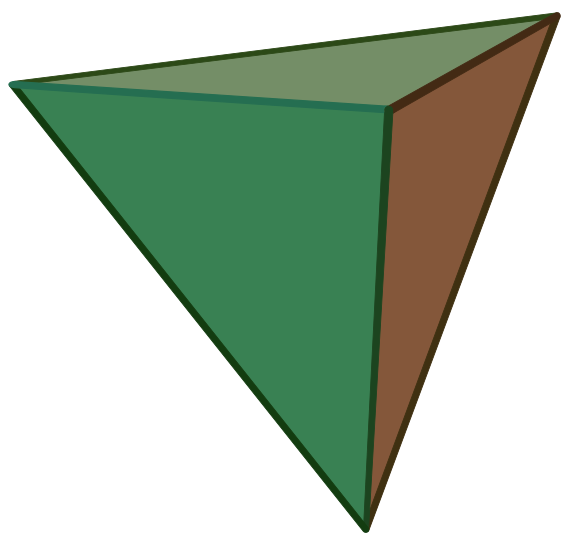
\includegraphics[width=0.25\marginparwidth]{SM/Tetrahedron.png}
\vspace*{-0.25cm}
\begin{center}\normalfont\small {Le Tétraèdre (le Feu).}\end{center}
\vspace*{-0.25cm}
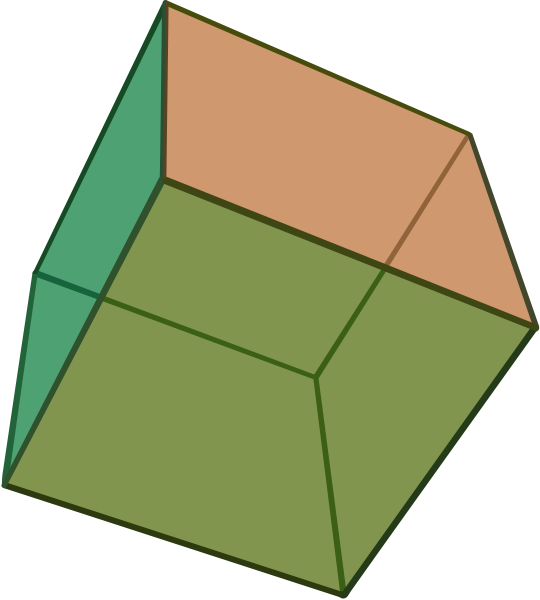
\includegraphics[width=0.25\marginparwidth]{SM/Hexahedron.png}
\vspace*{-0.25cm}
\begin{center}\normalfont\small {Le Cube (la Terre).}\end{center}
\vspace*{-0.25cm}
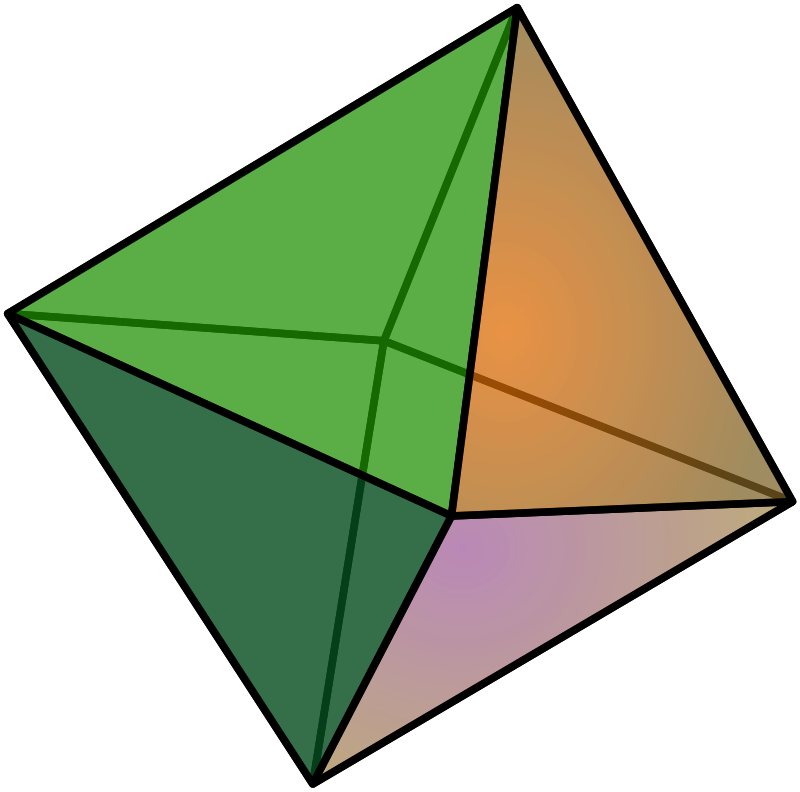
\includegraphics[width=0.25\marginparwidth]{SM/Octahedron.png}
\vspace*{-0.25cm}
\begin{center}\normalfont\small {L'Octaèdre (l'Air).}\end{center}
\vspace*{-0.25cm}
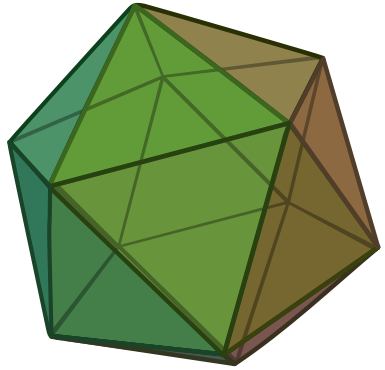
\includegraphics[width=0.25\marginparwidth]{SM/Icosahedron.png}
\vspace*{-0.25cm}
\begin{center}\normalfont\small {L'Icosaèdre (l'Eau).}\end{center}
\vspace*{-0.25cm}
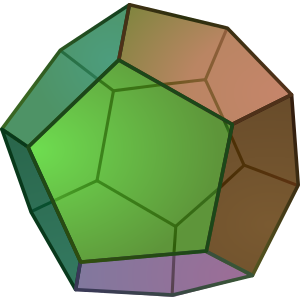
\includegraphics[width=0.25\marginparwidth]{SM/Dodecahedron.png}
\vspace*{-0.25cm}
\begin{center}\normalfont\small {Le Dodécaèdre (l'Univers).}\end{center}
\vspace*{-0.25cm}
\captionof{figure}{Les solides de Platon.}
\label{solides}
%\end{center}
}
De tout temps les hommes ont voulu comprendre et maîtriser la nature. Cette quête a amené de nombreux penseurs, et notamment les philosophes Grecs, à proposer des explications sur le monde qui nous entoure, et certaines de leurs idées se révéleront florissantes et donneront, des siècles plus tard, naissance à la Physique en tant que science au sens moderne du mot. 

\bsc{Anaxagore} ($\sim$\num{500}--\num{428} av.J.-C.) prônait que toute chose est formée de particules élémentaires. Cette idée sera reprise par \bsc{Empédocle} ($\sim$\num{495}--$\sim$\num{435} av.J.-C.) qui proposa l'eau, la terre, l'air et le feu comme étant ces particules. \bsc{Platon} (\num{428}/\num{427}--\num{348}/\num{347} av.J.-C.) associera ces quatre éléments aux polygones réguliers convexes de l'espace à trois dimensions (le tétraèdre pour le Feu, le cube pour la Terre, l'octaèdre pour l'Air, l'icosaèdre pour l'Eau, le dodécaèdre quant à lui représente l'Éther, élément constituant l'Univers (cf.Fig~\ref{solides})). On doit à \bsc{Leucippe} ($\sim$\num{460}--$\sim$\num{370} av.J.-C.) et son disciple \bsc{Démocrite} ($\sim$\num{460}--$\sim$\num{370} av.J.-C.) le concept d'atomes, indivisibles et séparés par du vide, qui composent la matière. La véracité de l'atomisme fera débat pendant plus de deux mille ans et ne sera validée expérimentalement qu'au cours du XIX\ieme siècle.

 Parmi les travaux les plus importants qui prouveront l'existence des atomes, citons ceux de \bsc{Lavoisier} (\num{1743}--\num{1794}) qui décompose de nombreuses substances en "Éléments". De multiples travaux sur les gaz, la cristallographie, la physique statistique et la thermodynamique. \bsc{Bernoulli} (\num{1700}--\num{1782}) : la cinétique des gaz, \bsc{Haüy} (\num{1743}--\num{1822}) : La forme des cristaux reflète la symétrie des "briques élémentaires" le constituant, \bsc{Dalton} (\num{1766}--\num{1844}) : symbolisation des corps simples et des corps composés par des symboles auxquels il donne un poids de matière (cf.Fig~\ref{atom}), et liste des masses atomiques d'un certain nombre d'éléments rapportées à la masse de l'hydrogène, \bsc{Gay-Lussac} (\num{1778}--\num{1850}) : les rapports des volumes des réactifs et des produits de réaction sont des nombres entiers petits, \bsc{Maxwell} (\num{1831}--\num{1879}) : dispersion statistique des vitesses des molécules, \bsc{Boltzmann} (\num{1844}--\num{1906}) : répartition statistique des vitesses dans un gaz, \bsc{Mendeleïev} : Classification périodique des éléments et prédiction de nouveaux atomes (cf.Fig~\ref{periodique}). Ces travaux feront passer petit à petit cette théorie en réalité scientifique. 
 
\marginpar
{
	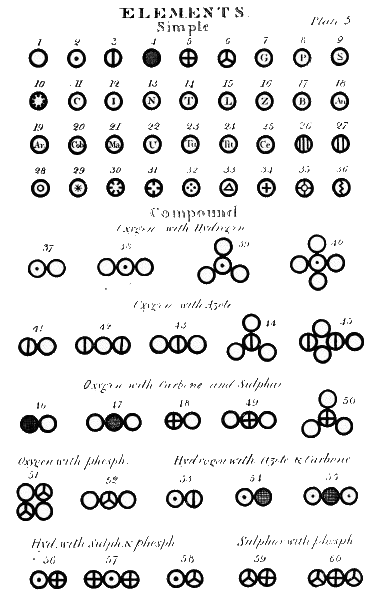
\includegraphics[width=\marginparwidth]{SM/Dalton.png}
    \captionof{figure}{Dessins de divers atomes et molécules tirés de l'ouvrage \textit{A New System of Chemical Philosophy}.}
    \label{atom}
}

\marginpar
{
	\vspace{2cm}
	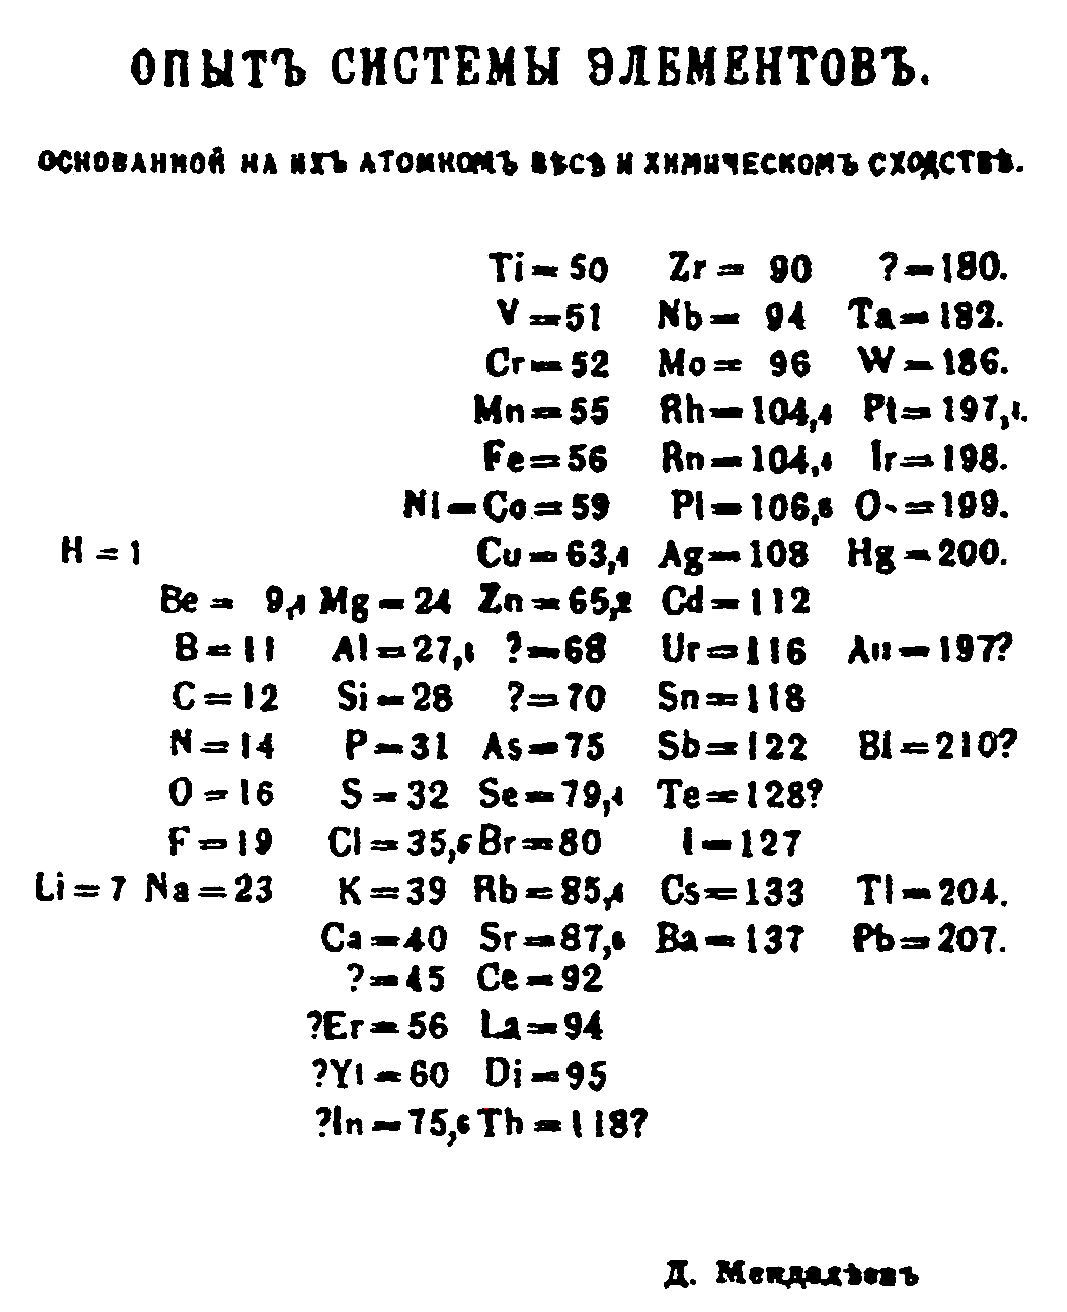
\includegraphics[width=\marginparwidth]{SM/periodique.png}
    \captionof{figure}{Tableau périodique de \bsc{Mendeleïev}.}
    \label{periodique}
}
D'autres domaines de la physique connaîtront des bouleversements importants au cours des siècles : 

Pour la mécanique et la cosmologie : \bsc{Copernic} (\num{1473}--\num{1543}) et \bsc{Galilée} (\num{1564}--\num{1642}) : Modèle héliocentrique, \bsc{Tycho Brahe} (\num{1546}--\num{1601}) : remise en cause de  l'immuabilité du monde supra-lunaire énoncée par \bsc{Aristote}, \bsc{Kepler} (\num{1571}--\num{1630}) : Orbite elliptique des planètes, \bsc{Newton} (\num{1643}--\num{1727}) : théorie de la gravitation universelle, \bsc{Lagrange} (\num{1736}--\num{1813}) et \bsc{Hamilton} (\num{1805}--\num{1865}) : Principe de moindre action, Lagrangien, Hamiltonien.

Pour l'électromagnétisme : \bsc{Coulomb} (\num{1736}--\num{1806}) : loi de \bsc{Coulomb}, \bsc{Volta} (\num{1745}--\num{1827}): pile voltaïque, \bsc{Ørsted} (\num{1777}--\num{1851}), \bsc{Ampère} (\num{1775}--\num{1836}), \bsc{Faraday} (\num{1792}--\num{1867}), \bsc{Henry} (\num{1797}--\num{1878}) : les phénomènes d'induction, \bsc{Maxwell} : Équations de Maxwell.

Avec la découverte de l'électron par \bsc{Thomson} (\num{1856}--\num{1940}) en \num{1887} qui fût prédit en \num{1874} par \bsc{Laming} et \bsc{Stoney}, \bsc{Thomson} développe le premier modèle de l'atome, qui est décrit comme une boule de charge nulle possédant un noyau positif avec des électrons négatifs (modèle du "\textit{plum-pudding}"). On découvre également durant cette période la radioactivité (\bsc{Becquerel} (\num{1852}--\num{1908})). La physique semble à cette époque complète et cohérente. Lord \bsc{Kelvin} dira même dans son discours à la " \textit{Royal Institution of Great Britain}" : \textit{"The beauty and clearness of the dynamical theory, which asserts heat and light to be modes of motion, is at present obscured by two clouds."}. Ces deux "nuages", l'incapacité à détecter l'éther luminifère  (expérience de \bsc{Michelson-Morley}) et la catastrophe ultraviolette du corps noir, donneront naissance respectivement à la relativité restreinte et à la mécanique quantique et feront entrer les physiciens dans la Physique Moderne.

Le début du siècle dernier sera une période florissante pour la physique des particules. \bsc{Planck} (\num{1858}--\num{1947}), afin de résoudre le problème du corps noir, proposera de quantifier les rayonnements : ceux-ci ne peuvent être qu'un multiple d'une constante qui porte son nom ($h$). \bsc{Einstein} (\num{1879}--\num{1955}) ira plus loin et expliquera durant l'\textit{Annus mirabilis} (\num{1905}) l'effet photoélectrique en proposant le photon comme quanta de lumière qui agit comme une particule. Il posera également les bases de la relativité restreinte cette même année, réfutant le concept d'éther. De nombreux physiciens vont ensuite poser les bases de la mécanique quantique: \bsc{Bohr} (\num{1885}--\num{1962}), \bsc{Compton} (\num{1892}--\num{1962}), \bsc{De Broglie} (\num{1892}--\num{1987}), \bsc{Schrödinger} (\num{1887}--\num{1961}), \bsc{Heisenberg} (\num{1901}--\num{1976}), \bsc{Dirac} (\num{1902}--\num{1984}), \bsc{Pauli} (\num{1900}--\num{1958}). Avec les progrès tant théoriques qu'instrumentaux de Physiciens tels que \bsc{Rutherford} (\num{1871}--\num{1937}), \bsc{Chadwick} (\num{1891}--\num{1974}), \bsc{Fermi} (\num{1901}--\num{1954}), qui explorent le monde subatomique, on découvre les deux forces (les forces faible et forte) agissant à l'échelle du subatomique qui s'ajoutent aux deux forces connues à l'époque (la force gravitationnelle et la force électromagnétique). Des physiciens tel \bsc{Schwinger} (\num{1918}--\num{1994}) veulent continuer la réunification des forces déjà avancée par les travaux de \bsc{Maxwell} (force électrique et magnétique). Dans les années \num{1960}, \bsc{Weinberg} (\num{1933}), \bsc{Salam} (\num{1926}--\num{1996}) et \bsc{Glashow} (\num{1932}), réunissent dans une théorie dite électrofaible les forces électromagnétique et faible. Cette théorie prédit trois bosons ($W^{+}$, $W^{-}$ et $Z^{0}$). Leur théorie nécessite un boson supplémentaire, le boson de \bsc{Higgs}, postulé en \num{1964} par \bsc{Brout}, \bsc{Englert}, \bsc{Higgs}, \bsc{Haggen}, \bsc{Guralnik} et \bsc{Kibble} afin de donner une masse aux particules. Cette théorie est la base du Modèle Standard de la physique des particules. La découverte des quarks amène à la création de la Chromodynamique Quantique (QCD) par \bsc{Politzer} (\num{1949}), \bsc{Wilczek} (\num{1951}), \bsc{Gross} (\num{1941}) afin de décrire l'interaction forte ; Cette dernière sera ensuite intégrée au Modèle Standard.

À partir de la seconde moitié du XX\ieme siècle, la Physique Subatomique a tenté de valider cette théorie et notamment par la découverte des bosons  $W^{+}$,$W^{-}$ et $Z^{0}$ en \num{1983}, du quarks top $t$ en \num{1995}, du neutrino tauique en \num{2000} et du boson de Higgs $H^{0}$ en \num{2012}. De nombreux efforts sont également menés afin de continuer l'unification des forces entre elles. On sait cependant que le Modèle Standard, bien que jamais mis en défaut, ne peut tout expliquer. Certaines questions restent ouvertes et cette théorie présente même quelques défauts. La technicouleur, des modèles avec des dimensions supplémentaires ou la Supersymétrie sont des théories d'extension du Modèle Standard. Mais aucune n'a pu être encore validée expérimentalement.

\section{Le Modèle Standard de la physique des particules}
 
Au début du siècle dernier, tout tendait à faire croire que le monde était simplement composé d'atomes; eux-mêmes constitués d'électrons tournant autour d'un noyau composé de protons et de neutrons. Tous les atomes connus avaient été soigneusement classés dans le tableau périodique de \bsc{Mendeleïev}. Cependant, grâce à l'invention d'accélérateurs de particules linéaires, cyclotrons (cf.Fig~\ref{cyclo}) puis synchrotrons et l'observation des rayons cosmiques, les physiciens découvrirent bientôt qu'une pléthore de particules instables pouvaient être créées durant des désintégrations. Les Physiciens tentèrent alors de créer et classer ces particules en utilisant des énergies de faisceau de plus en plus grandes. Ce qui amena à la découverte d'une sous structure au sein même des nucléons\footnote{Protons et neutrons.} qui composent le noyau : les quarks (\ref{structure}).
\marginpar
{
	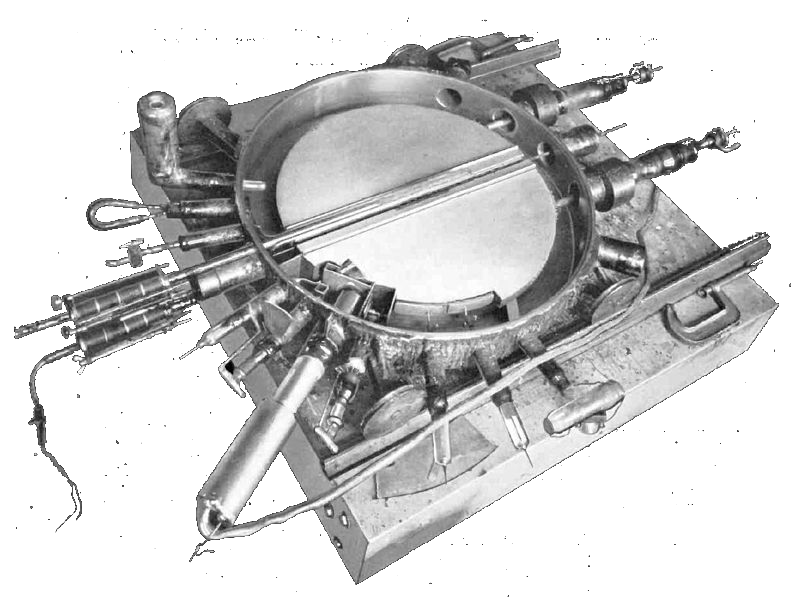
\includegraphics[width=\marginparwidth]{SM/cyclotron.png}
    \captionof{figure}{Cyclotron de \num{27} pouces, accélérateur de $^{2}$H à \SI{4}{\mega\eV} (Université de Berkley, \num{1932}).}
    \label{cyclo}
}

\vspace*{-0.5cm}
\begin{figure}[ht!]
\centering
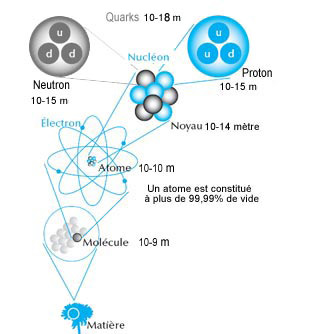
\includegraphics[width=0.50\textwidth]{SM/structure.jpg}
\captionof{figure}{Structure de la matière à différentes échelles.}
\label{structure}
\end{figure}

\vspace*{-0.5cm}
Parallèlement, de nouvelles interactions furent découvertes. Elles expliquaient les désintégrations radioactives ainsi que la cohésion des protons et des neutrons au sein du noyau atomique.

La physique des particules peut se résumer à la combinaison des deux démarches précédentes à savoir : trouver les particules élémentaires ainsi que les interactions fondamentales que ces particules peuvent subir. La manière dont ces particules interagissent est donnée par la formulation mathématique d'une théorie : le Modèle Standard.

\subsection{Les particules élémentaires}
Les particules élémentaires du Modèle Standard, supposées indivisibles\footnote{à ce jour}, peuvent être classées en deux catégories selon leur spin (une propriété quantique intrinsèque à chaque particule) :
\begin{itemize}[label=$\bullet$]
\item les \textit{fermions}, ils constituent la matière et sont de spin demi-entier.
\item les \textit{bosons}, ils sont les messagers de l'interaction et sont de spin entier.
\end{itemize}
Chaque particule du Modèle Standard possède des nombres quantiques telles que sa masse, sa charge électrique, en fraction de l'opposé de la charge électrique de l'électron $e$ par convention ($e=$\SI{602 176 565(35)e-19}{\coulomb}). Dans le cadre de la théorie, à chaque particule correspond une anti-particule\footnote{Une particule peut être sa propre anti-particule.} qui possède la même masse mais dont les nombres quantiques sont opposés.

\subsubsection{Les fermions}
Les fermions peuvent être classés en deux catégories selon qu'ils sont sensibles à l'interaction forte ou non. Dans le premier cas, ils font partie des \textit{quarks}, sinon ce sont des \textit{leptons}. Ces deux catégories sont elles-mêmes divisées en trois \textit{générations} (cf.Table~\ref{fermions}).

Les leptons ont une charge électrique entière (\num{-1}) pour les électrons, muons et taus, et une charge nulle pour les neutrinos électroniques, neutrinos muoniques et neutrinos tauiques.

Les quarks ont une charge électrique fractionnaire. On associe à chaque quark un nombre quantique appelé "couleur" (Rouge, Vert et Bleu). Dû à la propriété de confinement de couleur, un quark ne peut être isolé et doit se combiner avec un ou deux autres quarks afin de former respectivement des \textit{mésons} (cf.Fig~\ref{mesons}) et des \textit{baryons} (cf.Fig~\ref{baryons}). La somme des deux (trois) couleurs des quarks doit constituer un méson (baryon) "blanc" \footnote{Selon l'analogie avec la synthèse additive des couleurs.}. Les mésons et baryons sont regroupés sous le terme générique de \textit{hadrons}.

\marginpar
{
	\centering
	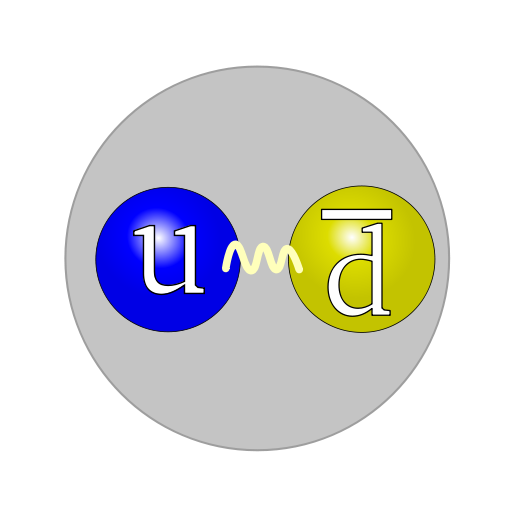
\includegraphics[width=\marginparwidth]{SM/quarks2.png}
	\captionof{figure}{Un méson ($\pi^{+}$).}
	\label{mesons}
}

\marginpar
{
	\centering
    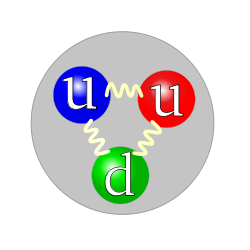
\includegraphics[width=\marginparwidth]{SM/quarks.png}
    \captionof{figure}{Un baryon ($p$).}
    \label{baryons}
}
	
\marginpar
{
	\centering
	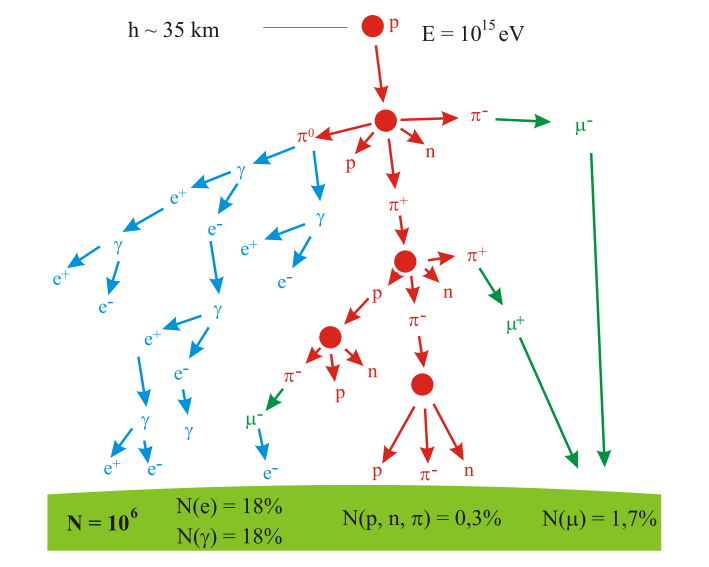
\includegraphics[width=0.95\marginparwidth]{SM/shower.png}
	\captionof{figure}{Schéma d'une gerbe atmosphèrique.}
	\label{gerbe}
}

La matière qui nous entoure n'est composée que de particules de la première génération. Tous les atomes sont composés d'électrons et de quarks $u$ et $d$ qui s'assemblent pour donner des protons $p$ et des neutrons $n$. Les autres particules peuvent être créées si l'énergie disponible est suffisante (lors de gerbe atmosphérique où un proton vient interagir avec des particules de notre atmosphère par exemple, figure \ref{gerbe}, ou dans un collisionneur).
\definecolor{Orange}{HTML}{FFDD00}
\definecolor{Orange2}{HTML}{FFC000}
\definecolor{Green}{HTML}{8FB73E}
\definecolor{Green2}{HTML}{4EA700}
\definecolor{Red}{HTML}{EF4123}
\definecolor{Red2}{HTML}{EF2300}
\vspace*{1cm}
\begin{table}[H]
	\centering
	\begin{tabular}{|O|O|O|O|N}
		\hline 
		\rowcolor{Orange2}Quarks & 1\iere génération & 2\ieme génération & 3\ieme génération \\
		\hline 
		\cellcolor{Orange2} Nom &\cellcolor{Orange} Up & \cellcolor{Orange} Charm &  \cellcolor{Orange} Top \\
		\cellcolor{Orange2} Notation &\cellcolor{Orange} $u$,$\bar{u}$ & \cellcolor{Orange} $c$,$\bar{c}$ &  \cellcolor{Orange} $t$,$\bar{t}$ \\
		\cellcolor{Orange2} Charge &\cellcolor{Orange} $\pm \frac{2}{3}$ & \cellcolor{Orange} $\pm \frac{2}{3}$ &  \cellcolor{Orange} $\pm \frac{2}{3}$ \\
		\cellcolor{Orange2} Masse &\cellcolor{Orange} \SI{0.005}{\giga\eV/\square\c} & \cellcolor{Orange} \SI{1.35}{\giga\eV/\square\c} &  \cellcolor{Orange} \SI{172.6}{\giga\eV/\square\c} \\
		\hline 
		\cellcolor{Orange2} Nom &\cellcolor{Orange} Down & \cellcolor{Orange} Strange &  \cellcolor{Orange} Bottom \\
		\cellcolor{Orange2} Notation &\cellcolor{Orange} $d$,$\bar{d}$ & \cellcolor{Orange} $s$,$\bar{s}$ &  \cellcolor{Orange} $b$,$\bar{b}$ \\
		\cellcolor{Orange2} Charge &\cellcolor{Orange} $\mp \frac{1}{3}$ & \cellcolor{Orange} $\mp \frac{1}{3}$ &  \cellcolor{Orange} $\mp \frac{1}{3}$ \\
		\cellcolor{Orange2} Masse &\cellcolor{Orange} \SI{0.01}{\giga\eV/\square\c}& \cellcolor{Orange} \SI{0.1}{\giga\eV/\square\c} &  \cellcolor{Orange} \SI{1.3}{\giga\eV/\square\c} \\
		\hline 
		\rowcolor{Green2} Leptons & 1\iere génération & 2\ieme génération & 3\ieme génération \\
		\hline
		\cellcolor{Green2} Nom & \cellcolor{Green} Électron & \cellcolor{Green} Muon & \cellcolor{Green} Tau \\
		\cellcolor{Green2} Notation & \cellcolor{Green} $e^{\pm}$ & \cellcolor{Green} $\mu^{\pm}$ & \cellcolor{Green} $\tau^{\pm}$ \\
		\cellcolor{Green2} Charge & \cellcolor{Green} $\pm$ \num{1} & \cellcolor{Green} $\pm$ \num{1} & \cellcolor{Green} $\pm$ \num{1} \\
		\cellcolor{Green2} Masse & \cellcolor{Green} \SI{0.511}{\mega\eV/\square\c} & \cellcolor{Green} \SI{105.7}{\mega\eV/\square\c}& \cellcolor{Green} \SI{1777}{\giga\eV/\square\c} \\
		\hline 
		\cellcolor{Green2} Nom & \cellcolor{Green} Neutrino électronique & \cellcolor{Green} Neutrino muonique & \cellcolor{Green} Neutrino tauique \\
		\cellcolor{Green2} Notation & \cellcolor{Green} $\nu_{e}$ & \cellcolor{Green} $\nu_{\mu}$ & \cellcolor{Green} $\nu_{\tau}$ \\
		\cellcolor{Green2} Charge & \cellcolor{Green} \num{0} & \cellcolor{Green} \num{0} & \cellcolor{Green} \num{0} \\
		\cellcolor{Green2} Masse & \cellcolor{Green} $<$\SI{0.017}{\mega\eV/\square\c} & \cellcolor{Green}$<$\SI{0.27}{\mega\eV/\square\c}  & \cellcolor{Green}$<$\SI{35}{\mega\eV/\square\c}\\
	\hline
\end{tabular} 
\captionof{table}{Fermions : Quarks et Leptons.}
\label{fermions}
\end{table}	

\subsubsection{Les bosons}
La description perturbative du Modèle Standard utilise l'échange de bosons virtuels, afin de décrire l'interaction entre deux particules. Les bosons sont les médiateurs des interactions. Les particules de matière (fermions) interagissent donc entre elles par l'échange de particules de spin \num{1} correspondant à la force responsable de leur interaction.
\smallskip
Chacune des quatre interactions possède donc un ou plusieurs bosons appelés bosons de jauge (bosons vecteurs) (cf.Table~\ref{bosons}) :

\marginpar
{
	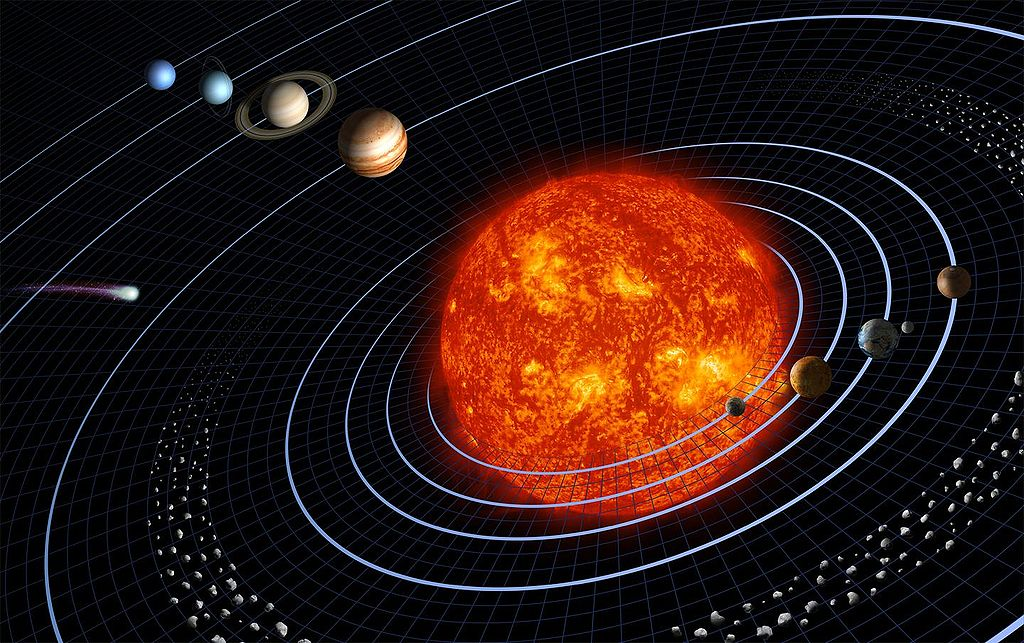
\includegraphics[width=\marginparwidth]{SM/solaire.jpg}
	\captionof{subfigure}{Gravité : Système solaire.}
	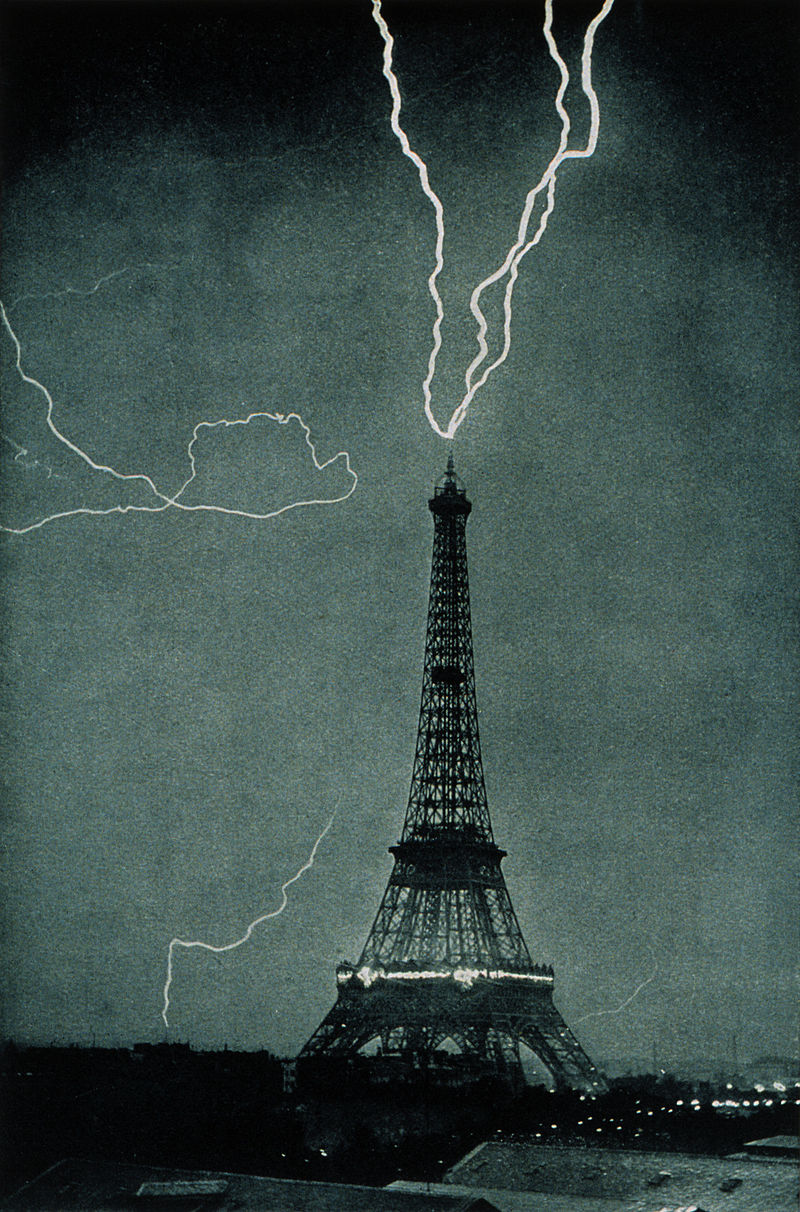
\includegraphics[width=\marginparwidth]{SM/foudre.jpg}
	\captionof{subfigure}{Électromagnétisme : la foudre.}
	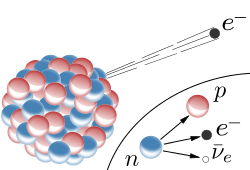
\includegraphics[width=\marginparwidth]{SM/beta.png}
	\captionof{subfigure}{Interaction faible : désintégration $\beta$.}
	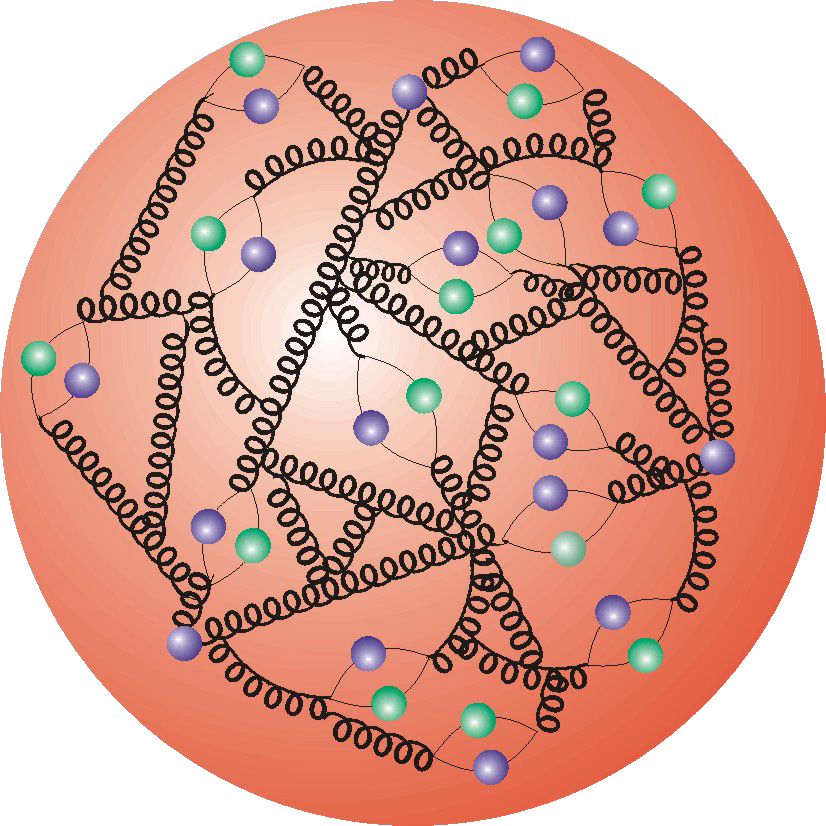
\includegraphics[width=0.8\marginparwidth]{SM/quarks3.png}
	\captionof{subfigure}{Interaction forte : confinement.}
	\captionof{figure}{Exemple d'effets des \num{4} interactions.}
}

\begin{itemize}[label=$\bullet$]
\item \textbf{L'interaction gravitationnelle} est la première à avoir été découverte et expliquée (\bsc{Galilée}, \bsc{Newton}). Elle est négligeable à l'échelle atomique. Elle est gouvernée par la masse des corps mise en jeu et elle domine à grande échelle (Univers, Galaxies, Planètes), son rayon d'action est infini. Sa description quantique repose sur un boson de spin \num{2} qui est encore activement recherché. Un pas décisif à été fait grâce à la détection par les expériences \textit{Laser Interferometer Gravitational-Wave Observatory} (LIGO) et Virgo des ondes gravitationnelles. Cette interaction est la seule à ne pas être intégrée au Modèle Standard. Elle est actuellement décrite par la relativité générale qui est une approche non quantique.

\item \textbf{L'interaction électromagnétique} gouverne les interactions entre les particules chargées. C'est l'une des interactions qui nous est la plus familière, puisque prépondérante dans notre vie quotidienne (lumière, chimie, frottements\ldots). Tout comme la gravité, son rayon d'action est infini. Son boson médiateur est le photon $\gamma$.

\item \textbf{L'interaction faible} à été découverte et comprise à travers la désintégration de particules avec changements de saveurs. Elle fait passer d'un fermion à un autre (par exemple lors de la désintégration $\beta$, elle transforme un neutron en un proton en changeant un quark $d$ en un quark $u$ avec la création d'un neutrino et d'un électron). Les bosons médiateurs de l'interaction sont les bosons $W^{+}$, $W^{-}$ et $Z^{0}$. Sa portée est de l'ordre de \SI{1e-18}{\meter} due à la masse des bosons médiateurs.

\item \textbf{L'interaction forte} permet l'échange de couleur entre les quarks, la création et l'annihilation de particules. Elle est responsable de la cohésion du noyau, et elle lie les nucléons entre eux à l'intérieur du noyau atomique. Ses bosons médiateurs, appelés gluons, sont au nombre de huit. Bien que ceux-ci soient supposés de masse nulle, la portée de l'interaction est de l'ordre de \SI{1e-15}{\meter}. Cette portée est la conséquence du principe de confinement de couleur qui affecte les quarks. En effet, cette interaction a la propriété de voir son intensité augmenter avec la distance, ce qui à tendance à regrouper les quarks entre eux. Cette propriété est également responsable du processus d'hadronisation des quarks et de la création de jets.
\end{itemize}

\vspace{1cm}
\begin{table}[ht!]
	\centering
	\begin{tabular}{|O|O|O|O|N}
		\hline 
		\rowcolor{Red2}Interaction&Rayon d'action&Bosons de jauge&Masses\\
		\hline 
		\cellcolor{Red}\shortstack{Forte}&
		\cellcolor{Red}\shortstack{\SI{2.5e-15}{\meter}}& 
		\cellcolor{Red}\shortstack{Gluons (\num{8})}&
		\cellcolor{Red}\shortstack{\num{0}}\\
		\hline 
		\cellcolor{Red}\shortstack{ Electromagnétique }&
		\cellcolor{Red}\shortstack{ $\infty$}& 
		\cellcolor{Red}\shortstack{Photon $\gamma$}&
		\cellcolor{Red}\shortstack{\num{0}}\\
		\hline 
		\cellcolor{Red}\shortstack{Faible}&
		\cellcolor{Red}\shortstack{\SI{10e-18}{\meter}}& 
		\cellcolor{Red}\shortstack{$W^{\pm}$,$Z^{0}$}&
		\cellcolor{Red}\shortstack{\num{80.399}, \SI{91.188}{\giga\eV/\square\c}}\\
		\hline 
		\cellcolor{Red}\shortstack{Gravitationnelle}&
		\cellcolor{Red}\shortstack{$\infty$}& 
		\cellcolor{Red}\shortstack{(Graviton)}&
		\cellcolor{Red}\shortstack{(inconnue)}\\
		\hline 
\end{tabular} 
\captionof{table}{Bosons : Interactions.}
\label{bosons}
\end{table}

\subsubsection{Le boson de Higgs}
Le boson de Higgs ($H^{0}$) est nécessaire afin de donner la masse des bosons $W^{\pm}$, $Z^{0}$ et des fermions. Bien que postulé en \num{1964}, il n'a été découvert qu'en \num{2012} par les expériences CMS et ATLAS. Contrairement aux bosons vecteurs, le boson de \bsc{Higgs} est de spin \num{0}.
\newpage
Toutes ces particules peuvent être résumées dans le tableau suivant : 

\begin{minipagewithmarginpars}[h]{\textwidth}
	\vspace{-0.5cm}
	\centering
	\hspace*{-1.5cm}
	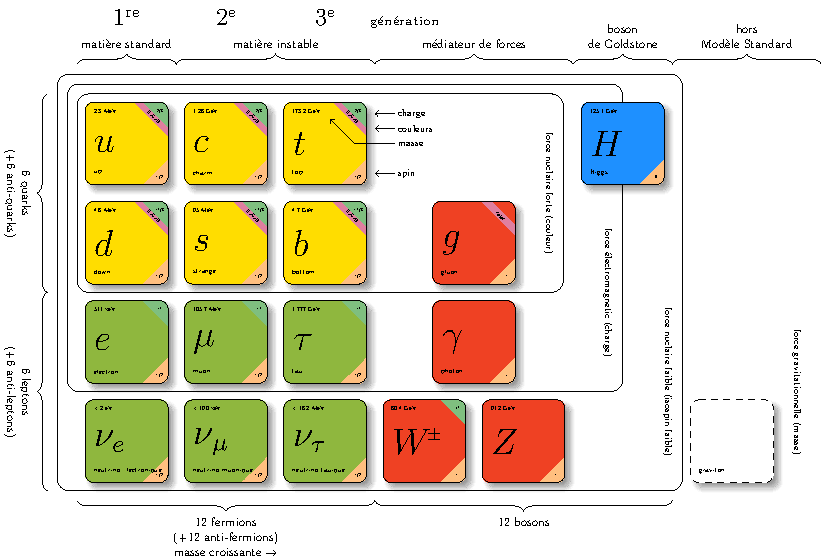
\includegraphics[scale=1]{SM/bestiaire.pdf}
	%\includestandalone{./SM/bestiaire}
	\captionof{figure}{Classification des quarks, leptons et bosons.}
	\label{bestiaire}
\end{minipagewithmarginpars}
\subsection{Le formalisme du Modèle Standard}
\marginpar
{
	\centering
	%	\vspace*{1.5cm}
	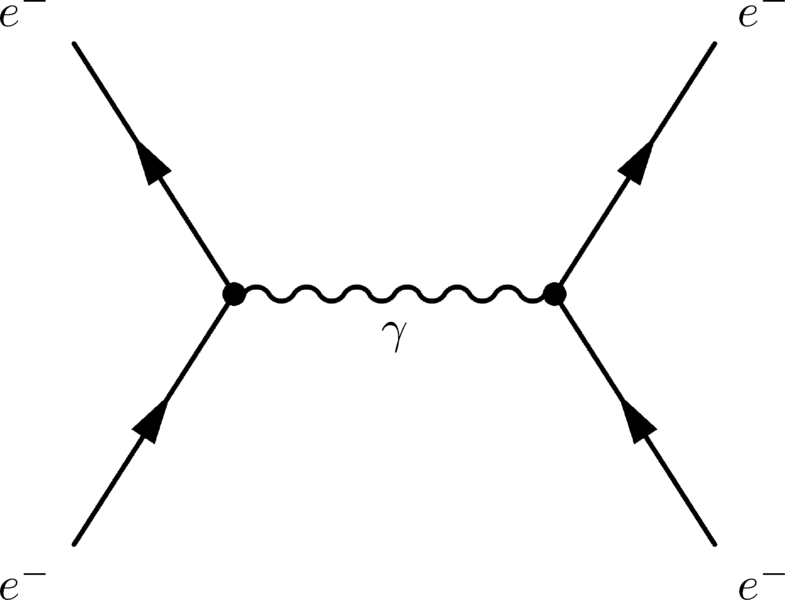
\includegraphics[width=\marginparwidth]{SM/feyn0.png}
	\captionof{subfigure}{Développement à l'arbre.}
	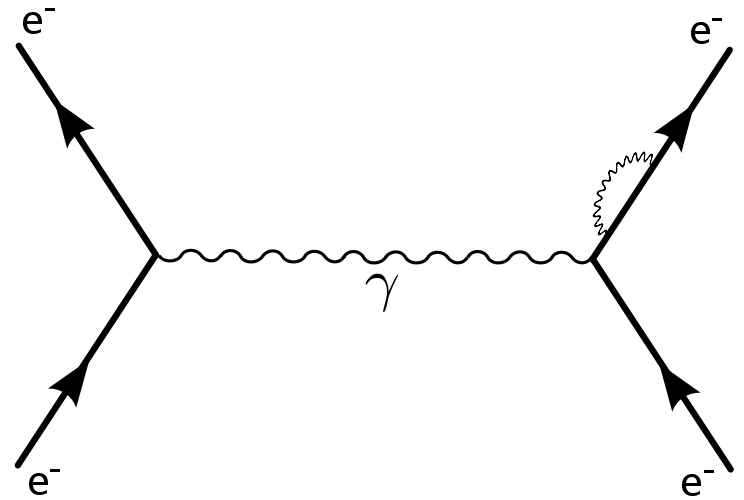
\includegraphics[width=\marginparwidth]{SM/feyn1.png}
	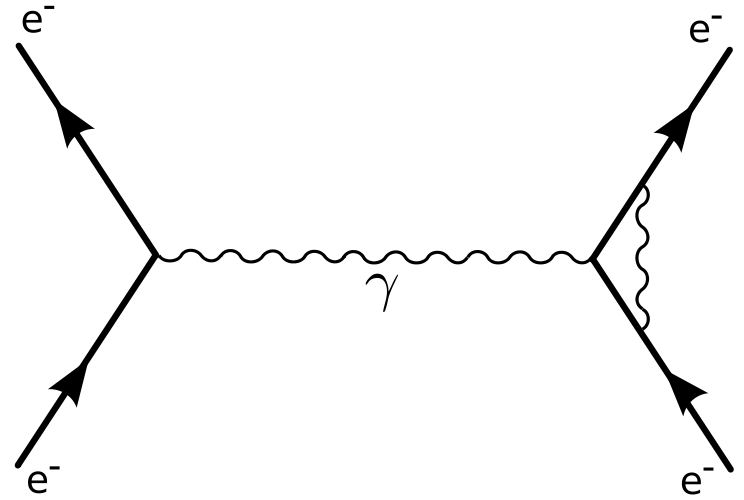
\includegraphics[width=\marginparwidth]{SM/feyn2.png}
	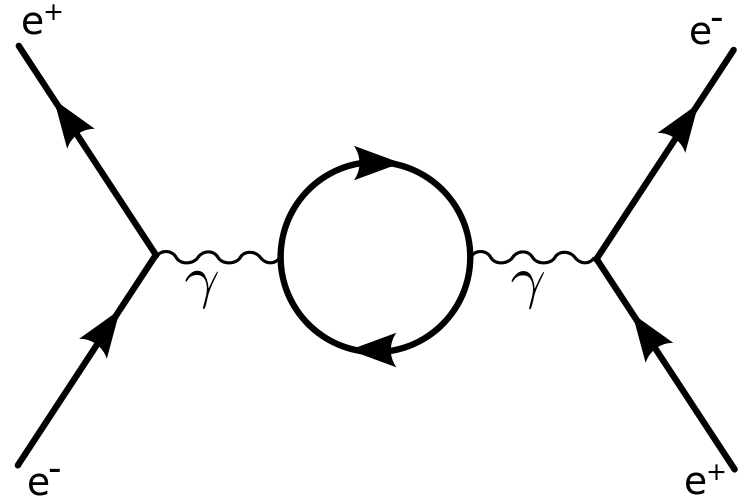
\includegraphics[width=\marginparwidth]{SM/feyn3.png}
	\captionof{subfigure}{Développement à l'ordre \num{1}.}
	\captionof{figure}{Exemple de diagrammes de Feynman pour le développement en série de la diffusion électron-électron.}
	\label{feyn}
}
Le Modèle Standard est une théorie non-abélienne où les interactions sont régies par des symétries locales de jauge. Elle repose sur la théorie quantique des champs qui permet de décrire les particules et leurs interactions. Cette théorie est à la fois quantique et relativiste. Elle permet donc de caractériser les interactions par des probabilités de transition d'un état initial à un état final, ainsi que de rendre compte du temps de propagation des interactions, la description des particules à haute énergie et les créations et annihilation de particules.

Dans cette théorie, à chaque type de particule est associé un champ $\psi(\vec{x},t)$ et les interactions sont liées à des propagateurs. La création (l'annihilation) de particules est associée à des opérateurs qui excitent (désexcitent) le champ de particules à une position $\vec{x}$ et à un temps $t$. L'un des postulats de la théorie quantique des champs est que l'ensemble des informations de la théorie est contenu dans un Lagrangien $\mathcal{L}$ qui s'exprime en fonction des champs et de leurs dérivées. Il est possible, à partir de ce Lagrangien d'obtenir les équations du mouvement en minimisant son action $S=\int\mathcal{L}\Diff4{x}$.
Le Modèle Standard est une théorie perturbative, c'est-à-dire que les observables sont calculées par une méthode qui s'appuie sur un développement en série dont la précision augmente avec l'ordre. Au premier ordre, l'observable est dite "être calculée à l'arbre" ou \textit{Leading Order} (LO). Ce développement en série n'est valable que si les constantes de couplage des interactions restent faibles devant l'unité. Ce développement en série peut être schématisé grâce aux diagrammes de \bsc{Feynmann} (cf.Fig~\ref{feyn}), qui représentent des règles de calculs. Chaque type de particule et d'interaction possède son symbole et à chaque particule doit être connecté un vertex (représentant une interaction).

Le principe selon lequel les interactions sont gouvernées par des symétries est également un postulat important du Modèle Standard. De par le théorème de \bsc{Noether}, les symétries continues sont liées à des quantités physiques qui se conservent. Le Modèle Standard est basé sur le produit direct du groupe de la chromodynamique quantique, décrivant l'interaction forte, qui impose une conservation de la charge de couleur, $SU(3)_{C}$ et du groupe de la théorie électrofaible, $SU(2)_{L} \otimes U(1)_{Y}$, imposant une symétrie locale de l'isospin $I$ associé au groupe $SU(2)_{L}$ et une symétrie locale de l'hypercharge $Y$ du groupe $U(1)_{Y}$.

\subsection{Lagrangien du Modèle Standard}
Le Modèle Standard est une théorie de jauge qui se base sur le groupe $SU(3)_{C} \otimes SU(2)_{L} \otimes U(1)_{Y}$ dont le lagrangien peut s'écrire sous la forme :

\begin{equation}
\mathcal{L_{MS}}=\mathcal{L}_{\mathrm{Yang-Mills}}+\mathcal{L}_{\mathrm{Dirac}}+\mathcal{L}_{\mathrm{Yukawa}}+\mathcal{L}_{\mathrm{Higgs}}
\end{equation}

\subsubsection{Le terme de \bsc{Yang-Mills} (secteur de jauge)}
Le secteur de jauge est la partie cinématique des champs de jauge :
\begin{equation}
\mathcal{L}_{\mathrm{Yang-Mills}}=-\frac{1}{4}B_{\mu\nu}B^{\mu\nu}-\frac{1}{4}W_{\mu\nu}^{a}W_{a}^{\mu\nu}-\frac{1}{4}G_{\mu\nu}^{A}G_{A}^{\mu\nu}
\end{equation}
où 
\begin{equation}
B_{\mu\nu}=\partial_{\mu}B_{\nu}-\partial_{\nu}B_{\mu}
\end{equation}
avec $B_{\mu}$ le champ isoscalaire associé au groupe d'hypercharge $U(1)_{Y}$,
\begin{equation}
W_{\mu\nu}^{a}=\partial_{\mu}W_{\nu}^{a}-\partial_{\nu}W_{\mu}^{a}+g\epsilon_{abc}W_{\mu}^{b}W_{\nu}^{c}
\end{equation}
où $W_{\mu}^{a} (a=1,2,3)$ est le triplet d'isospin $I=\num{1}$ du groupe de l'isospin faible $SU(2)_{L}$, $g$ la constante de couplage de l'isospin faible et $\epsilon_{abc}$ les constantes de structures antisymétriques correspondantes.  
\begin{equation}
G_{\mu\nu}^{A}=\partial_{\mu}G_{\nu}^{A}-\partial_{\nu}G_{\mu}^{A}+g'f_{ABC}G_{\mu}^{B}G_{\nu}^{C}
\end{equation}
les champs des gluons $G_{\mu}^{A} (A=1,2,..,8)$, bosons vecteurs de $SU(3)_{c}$, $g'$ la constante de couplage de couleur et $f_{ABC}$ les constantes de structures de $SU(3)_{C}$.
La nature non-abélienne de $SU(2)_{L}$ et $SU(3)_{c}$ amène à des termes supplémentaires dans l'écriture des champs du triplet d'isospin et des champs de gluons. Ce sont ces termes qui sont responsables de l'interaction des bosons $W$ et des gluons $g$.

\subsubsection{Le secteur de \bsc{Dirac}}
Le secteur de \bsc{Dirac} décrit les interactions des fermions avec les bosons de jauge. Dans le secteur électrofaible, les fermions se regroupent de manière asymétrique dans des doublets d'isospin faible de chiralité gauche et dans des singulets de chiralité droite (cf.Table~\ref{doublets}). Il y a violation maximale de la parité de $SU(2)_{L}\otimes U(1)_{Y}$

\begin{table}[H]
	\centering
	\begin{tabular}{|L|L|} 
	\hline
	\rowcolor{Orange2}\multicolumn{2}{|Cc|}{Quarks} \\
	\hline
	Gauches $Q_{\alpha L}^{i}$ & $
	\left(\begin{matrix} 
	 u^{i}\\
	 d^{i} 
	\end{matrix}\right)_{L}$,$\ 
	\left(\begin{matrix} 
	 c^{i}\\
	 s^{i}
	\end{matrix}\right)_{L}$,$\ 
	\left(\begin{matrix} 
	 t^{i}\\
	 b^{i}
	\end{matrix}\right)_{L}$ \\
	\hline
	Droits $Q_{\beta R}^{i}$&$ u_{iR},\ d_{iR},\ c_{iR},\ s_{iR},\ t_{iR},\ b_{iR}$\\
	\hline
	\rowcolor{Green2}\multicolumn{2}{|Cc|}{Leptons} \\
	\hline
	Gauche $L_{\alpha L}$& $
	\left(\begin{matrix} 
	\nu_{e}\\
	 e^{-}
	\end{matrix}\right)_{L}$,$\ 
	\left(\begin{matrix} 
	\nu_{\mu}\\
	\mu
	\end{matrix}\right)_{L}$,$\ 
	\left(\begin{matrix} 
	\nu_{\tau}\\
	\tau
	\end{matrix}\right)_{L} $\\
	\hline
	Droits $L_{\gamma R}$& $e^{-}_{R},\ \mu_{R},\ \tau_{R},\ \left(\nu_{e R},\ \nu_{\mu R},\ \nu_{\tau R}\right)$ \\
	\hline
\end{tabular}
\captionof{table}{Doublets et singulets pour $SU(2)_{L}$ ; $i=\left\{\num{1},~\num{2},~\num{3}\right\}$ couleurs, $\alpha=\left\{\num{1},~\num{2},~\num{3}\right\}$ familles, $\beta=\left\{u,~d,~s,~c,~t,~b~\right\}$, $\gamma=\left\{e^{-},~\mu,~\tau,~\left(\nu_{e},~\nu_{\mu},~\nu_{\tau}\right)\right\}$.}
\label{doublets}
\end{table}	

En suivant ces notations le secteur de \bsc{Dirac} du Lagrangien du Modèle Standard s'écrit:
\marginpar
{
\begin{equation*}
\sigma_{1}=\begin{pmatrix} 
0&1\\
1&0\\
\end{pmatrix}
\end{equation*}
\vspace{0.2cm}
\begin{equation*}
\sigma_{2}=\begin{pmatrix} 
0&-i\\
i&0\\
\end{pmatrix}
\end{equation*}
\vspace{0.2cm}
\begin{equation*}
\sigma_{3}=\begin{pmatrix} 
1&0\\
0&-1\\
\end{pmatrix}
\end{equation*}
\captionof{figure}{Les matrices canoniques de \bsc{Pauli}.}
\label{Pauli}
}
\marginpar
{
\begin{equation*}
\lambda_{1}=\begin{pmatrix} 
0&1&0\\
1&0&0\\
0&0&0
\end{pmatrix}
\end{equation*}
\vspace{0.2cm}
\begin{equation*}
\lambda_{2}=\begin{pmatrix} 
0&-i&0\\
i&0&0\\
0&0&0
\end{pmatrix}
\end{equation*}
\vspace{0.2cm}
\begin{equation*}
\lambda_{3}=\begin{pmatrix} 
1&0&0\\
0&-1&0\\
0&0&0
\end{pmatrix}
\end{equation*}
\vspace{0.2cm}
\begin{equation*}
\lambda_{4}=\begin{pmatrix} 
0&0&1\\
0&0&0\\
1&0&0
\end{pmatrix}
\end{equation*}
\vspace{0.2cm}
\begin{equation*}
\lambda_{5}=\begin{pmatrix} 
0&0&-i\\
0&0&0\\
i&0&0
\end{pmatrix}
\end{equation*}
\vspace{0.2cm}
\begin{equation*}
\lambda_{6}=\begin{pmatrix} 
0&0&0\\
0&0&1\\
0&1&0
\end{pmatrix}
\end{equation*}
\vspace{0.2cm}
\begin{equation*}
\lambda_{7}=\begin{pmatrix} 
0&0&0\\
0&0&-i\\
0&i&0
\end{pmatrix}
\end{equation*}
\vspace{0.2cm}
\begin{equation*}
\lambda_{8}=\frac{1}{\sqrt{3}}\begin{pmatrix} 
1&0&0\\
0&1&0\\
0&0&-2
\end{pmatrix}
\end{equation*}
\captionof{figure}{Les matrices canoniques de \bsc{Gell-Mann}.}
\label{Gell-Mann}
}

\begin{equation}
\begin{split}
\mathcal{L}_{\mathrm{Dirac}}=&i\sum_{\alpha=1}^{3}\bar{L}_{\alpha L}\gamma_{\mu}D_{L_{L}}^{\mu}L_{\alpha L}+\sum_{\gamma=1}^{3(6)}\bar{L}_{\gamma R}\gamma_{\mu}D_{L_{R}}^{\mu}L_{\gamma R}\\
&+\sum_{\alpha=1}^{3}\sum_{i=1}^{3}\bar{Q}_{\alpha L}^{i}\gamma_{\mu}D_{Q_{L}}^{\mu}Q_{\alpha L}^{i}+\sum_{\beta=1}^{6}\sum_{i=1}^{3}\bar{Q}_{\beta R}^{i}\gamma_{\mu}D_{Q_{R}}^{\mu}Q_{\beta R}^{i}
\end{split}
\end{equation}
Avec les dérivées covariantes de la forme : 
\begin{equation}
D_{\mu L_{L}}=\partial_{\mu} -ig\frac{\sigma^a}{2}W_{\mu}^{a}-ig'\frac{Y^{W}_{L}}{2}B_{\mu}
\end{equation}
\begin{equation}
D_{\mu L_{R}}=\partial_{\mu} -ig'\frac{Y^{W}_{R}}{2}B_{\mu}
\end{equation}
\begin{equation}
D_{\mu Q_{L}}=\partial_{\mu} -ig\frac{\sigma^a}{2}W_{\mu}^{a}-ig'\frac{Y^{W}_{L}}{2}B_{\mu}-ig''\frac{\lambda^{A}}{2}Q_{\mu}^{A}
\end{equation}
\begin{equation}
D_{\mu Q_{R}}=\partial_{\mu}ig'\frac{Y^{W}_{R}}{2}B_{\mu}-ig''\frac{\lambda^{A}}{2}Q_{\mu}^{A}
\end{equation}
où $\sigma^{a}$ sont les générateurs de $SU(2)_{L}$ (matrices de Pauli (cf.Fig.~\ref{Pauli})), $\lambda^{A}$ les générateurs de $SU(3)_{c}$ (matrices de Gell-Mann (cf.Fig.~\ref{Gell-Mann})) et $Y^{W}$, l'hypercharge faible, le générateur de $U(1)_{Y}$. 
Afin d'obtenir les charges électriques pour chaque fermion, on pose:
\begin{multline}
\begin{split}
&Y^W(L_{\alpha L})=-1,\ &Y^W(e_{R},\mu_{R},\tau_{R})=-2,\ &\left(Y^W(\nu_{e R},\nu_{\mu R},\nu_{\tau R})=0\right)\\
&Y^W(Q_{\alpha L})=\frac{1}{3},\ &Y^W(u_{R},c_{R},t_{R})=\frac{4}{3},\ &Y^W(d_{R},s_{R},b_{R})=-\frac{2}{3}
\end{split}
\end{multline}  


\subsubsection{Le secteur de \bsc{Higgs}} 
La symétrie électrofaible est incompatible avec la description de fermions massifs. En effet, dans le Lagrangien les termes de masse des fermions sont de la forme 
\begin{equation}
\mathcal{L_{M}}=-m\bar{\phi}\phi=-m \left(\phi_{L}^{\dagger}\phi_{R}+\phi_{R}^{\dagger}\phi_{L}\right)
\end{equation}
Cependant, ces termes brisent la symétrie $SU(2)$ et ne sont donc pas inclus dans le Lagrangien. De plus, l'expérience montre que les bosons de jauge $W$ doivent posséder une masse. Or l'introduction des termes de masse pour ces bosons est également impossible pour les mêmes raisons.

Afin de résoudre ces problèmes, on introduit un champ scalaire complexe $\phi$, doublet de $SU(2)_{L}$ de quatre champs réels $\phi_{i}$ et d'hypercharge $Y=1$ :
\begin{equation}
\phi=\begin{pmatrix} 
\phi^{+}\\
\phi^{0}
\end{pmatrix}=\frac{1}{\sqrt{2}}\begin{pmatrix} 
\phi_{1}+\phi_{2}\\
\phi_{3}+\phi_{4}
\end{pmatrix}
\end{equation}
On utilise l'expression du Lagrangien la plus générale pour un champ scalaire complexe de $SU(2)$:
\begin{equation}
\mathcal{L}_{\mathrm{Higgs}}=\left(D_{\mu}\phi\right)^{\dagger}\left(D^{\mu}\phi\right)-V(\phi),
\end{equation}
avec 
\begin{equation}
D_{\mu}=\partial_{\mu} -ig\frac{\sigma^a}{2}W_{\mu}^{a}-ig'\frac{Y}{2}B_{\mu}.
\end{equation}
Afin que le lagrangien $\mathcal{L}_{\mathrm{Higgs}}$ soit invariant globalement, le potentiel scalaire $V(\phi)$ ne doit pas comporter de puissances impaires de $\phi$. De plus, afin que la théorie reste renormalisable, les puissances au delà de $\phi^4$ sont à proscrire.

Le potentiel $V(\phi)$ est donc de la forme :
\begin{equation}
V(\phi)=\mu^{2}\phi^{\dagger}\phi+\lambda\left(\phi^{\dagger}\phi\right)^2,
\end{equation}
et a un profil différent selon les signes de $\mu^{2}$ et de $\lambda$ (Fig. \ref{profile}).
\marginpar{ 
\resizebox {\marginparwidth} {!} 
{
%\begin{tikzpicture}
%\begin{axis}[view={15}{15},yticklabels={,,},xticklabels={,,},zticklabels={,,},mesh/interior colormap name=hot,colormap/blackwhite]
%\addplot3[surf,shader=faceted,samples=30,fill opacity=0.5,opacity=0.4,domain=0:1.05,y domain=0:2*pi,z buffer=sort]({x * cos(deg(y))}, {x * sin(deg(y))}, {-x*x-x*x*x*x});
%\end{axis}
%\end{tikzpicture}
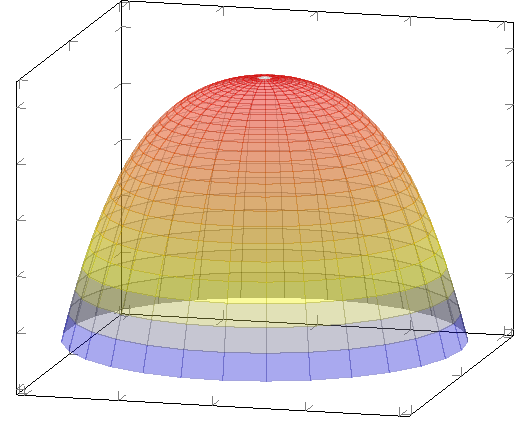
\includegraphics[scale=1]{SM/mm.pdf}
}
\captionof{subfigure}{$\mu^{2}<0$, $\lambda<0$.}
\resizebox {\marginparwidth} {!} 
{
%\begin{tikzpicture}
%\begin{axis}[view={15}{15},yticklabels={,,},xticklabels={,,},zticklabels={,,},mesh/interior colormap name=hot,colormap/blackwhite]
%\addplot3[surf,shader=faceted,samples=30,fill opacity=0.5,opacity=0.4,domain=0:1.05,y domain=0:2*pi,z buffer=sort]({x * cos(deg(y))}, {x * sin(deg(y))}, {+x*x+x*x*x*x});
%\end{axis}
%\end{tikzpicture}
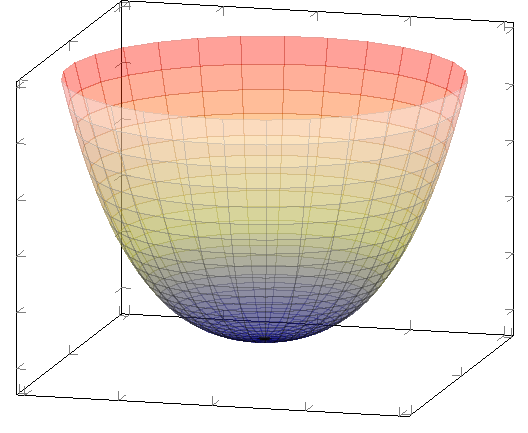
\includegraphics[scale=1]{SM/pp.pdf}
}
\captionof{subfigure}{$\mu^{2}>0$, $\lambda>0$.}
\resizebox {\marginparwidth} {!} 
{
%\begin{tikzpicture}
%\begin{axis}[view={15}{15},yticklabels={,,},xticklabels={,,},zticklabels={,,},mesh/interior colormap name=hot,colormap/blackwhite]
%\addplot3[surf,shader=faceted,samples=30,fill opacity=0.5,opacity=0.4,domain=0:1.05,y domain=0:2*pi,z buffer=sort]({x * cos(deg(y))}, {x * sin(deg(y))}, {+x*x-x*x*x*x});
%\end{axis}
%\end{tikzpicture}
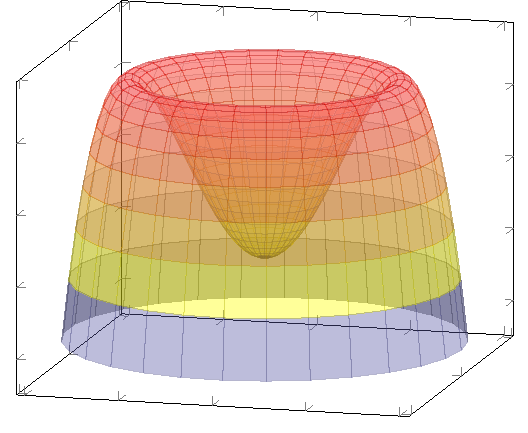
\includegraphics[scale=1]{SM/pm.pdf}
}
\captionof{subfigure}{$\mu^{2}>0$, $\lambda<0$.}
\resizebox {\marginparwidth} {!} 
{
	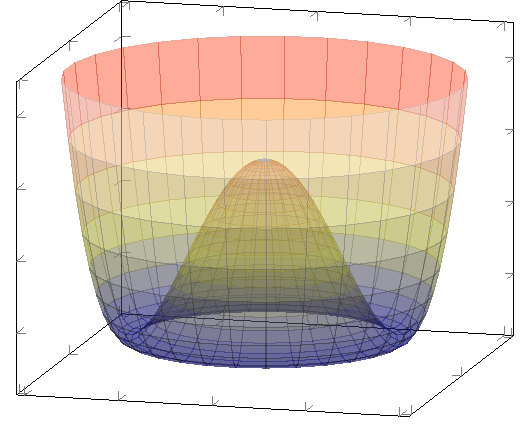
\includegraphics[scale=1]{SM/mp.pdf}
}
%\begin{tikzpicture}
%\begin{axis}[view={15}{15},yticklabels={,,},xticklabels={,,},zticklabels={,,},mesh/interior colormap name=hot,colormap/blackwhite]
%\addplot3[surf,shader=faceted,samples=30,fill opacity=0.5,opacity=0.4,domain=0:1.05,y domain=0:2*pi,z buffer=sort]({x *cos(deg(y))},{x*sin(deg(y))},{-x*x+x*x*x*x});
%\end{axis}
%\end{tikzpicture}
\captionof{subfigure}{$\mu^{2}<0$, $\lambda>0$.}
\captionof{figure}{Les différents profils de $V(\phi)$ selon les signes de $\mu^{2}$ et $\lambda$.}
\label{profile}
}
Les cas où $\mu^{2}>0$ ne possèdent qu'un minimum en $0$ sont inutiles. Le cas $\lambda<0$ n'est pas stable. Il ne reste plus que le cas où $\mu^{2}<0$ et $\lambda>0$, figure \ref{pot}.

\begin{minipagewithmarginpars}[h]{0.95\textwidth}
\centering
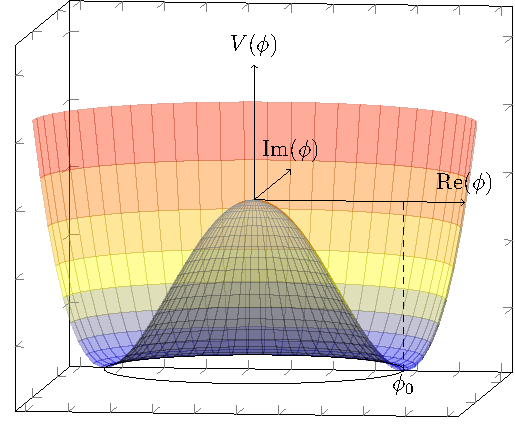
\includegraphics[scale=1]{SM/good.pdf}
%\begin{tikzpicture}
%\begin{axis}[view={7}{7},yticklabels={,,},xticklabels={,,},zticklabels={,,},mesh/interior colormap name=hot,colormap/blackwhite,]
%\addplot3[surf,shader=faceted,samples=30,fill opacity=0.5,opacity=0.4,domain=0:1.05,y domain=0:pi,z buffer=sort]({x * cos(deg(y))}, {x * sin(deg(y))}, {-x*x+x*x*x*x});
%\addplot3[->] coordinates{(0,0,0) (0,0,0.2)}node[above] {$V(\phi)$};
%\addplot3[->] coordinates{(0,0,0) (1.0,0,0)}node[above] {$\Re(\phi)$};
%\addplot3[->] coordinates{(0,0,0) (0,1.5,0)}node[above] {$\Im(\phi)$};
%\addplot3[color=black,samples=50,domain=0:2*pi,line width=0.2pt, line cap =round,]({sqrt(0.5)*cos(deg(x))},{sqrt(0.5)*sin(deg(x))},{-0.25});
%\addplot3[dashed]coordinates{(sqrt(0.5),0,-0.25) (sqrt(0.5),0,0)};
%\node (A) at (axis cs:0.70710678118,0,-0.27){$\phi_{0}$};
%\end{axis}
%\end{tikzpicture}
\captionof{figure}{Potentiel $V(\phi)$ pour $\mu^{2}<0$ et $\lambda>0$.}
\label{pot}
\end{minipagewithmarginpars}

Le potentiel est donc métastable pour $\phi$=0, et les minima sont situés sur un cercle de rayon $v=\sqrt{\frac{\mu^{2}}{\lambda}}$. On peut prendre par exemple :
\begin{equation}
H_{0}=\frac{1}{\sqrt{2}}\begin{pmatrix} 
0\\
v
\end{pmatrix} \, v=\sqrt{\frac{\mu^{2}}{\lambda}}
\end{equation}
et en développant le doublet $H$ autour de cet état du champ de \bsc{Higgs} qui brise la symétrie $SU(2)_{L}\otimes U(1)_{Y}$ on trouve : 
\begin{equation}
H=\frac{1}{\sqrt{2}}\exp^{-i\Theta_{a}T_{a}}\begin{pmatrix} 
0\\
h+v
\end{pmatrix}=\frac{1}{\sqrt{2}}\begin{pmatrix} 
i\phi_{1}+\phi{2}\\
h+v-i\phi_{3}
\end{pmatrix}
\end{equation}
où $v=\SI{246}{\giga\eV}$ est la densité moyenne d'énergie du vide, $T^{a}$ ($a=$\num{1}, \num{2}, \num{3}), les générateurs de $SU(2)_{L}$ et $\Theta_{a}$ sont les trois champs de \bsc{Goldstone} de masse nulle qui apparaissent lors de la brisure de la symétrie continue.

Il est possible de définir les bosons $W_{\mu}^{\pm}$,$Z_{\mu}^{0}$,$\gamma_{\mu}$ et $\phi^{\pm}$ 
\begin{equation}
\begin{split}
W_{\mu}^{\pm}&=\frac{W_{\mu}^{1}\mp iW_{\mu}^{2}}{\sqrt{2}}\, \ Z_{\mu}^{0}=-B_{\mu}\sin(\theta_{W})+W_{\mu}^{3}\cos(\theta_{W})\\
\gamma_{\mu}&=B_{\mu}\cos(\theta_{W})+W_{\mu}^{3}\sin(\theta_{W})\, \ \phi^{\pm}=\frac{\phi_{1}\mp i\phi_{2}}{\sqrt{2}}
\end{split}
\end{equation}
qui correspondent aux bosons $W^{\pm}$, $Z^{0}$ et $\gamma$ et au scalaire chargé du champ de \bsc{Higgs}. En choisissant une jauge unitaire, les bosons de \bsc{Goldstone} sont absorbés pour donner les composantes longitudinales des bosons $W^{\pm}$ et $Z^{0}$. Le boson de Higgs acquiert donc sa masse par auto-couplage et les bosons de jauge par interaction avec le champ de \bsc{Higgs}.

L'interaction est contenue dans la partie cinétique du Lagrangien du secteur de \bsc{Higgs} et donne les masses suivantes : 
\begin{equation}
m_{W^{\pm}}=\frac{g''v}{2} \quad m_{Z_{0}}=\frac{\sqrt{g''^{2}+g'^{1}}}{2}v \quad m_{\gamma}=0 
\end{equation} 
La théorie ne donne aucun indice sur la constante de couplage $\lambda$, la masse du boson de \bsc{Higgs} ne peut donc pas être déduite. La recherche de ce boson a été une priorité pendant plusieurs décennies. Ce n'est qu'en \num{2012}, grâce aux détecteurs CMS et ATLAS, que l'on a prouvé l'existence du boson de \bsc{Higgs} et que sa masse (\SI{125.9}{\giga\eV}) a pu être reconstruite. 

\subsubsection{Le secteur de \bsc{Yukawa}}
Le secteur de \bsc{Yukawa} décrit l'interaction entre le champ de Higgs et les champs de fermions.
\begin{equation}
\begin{split}
\mathcal{L}_{\mathrm{Yukawa}}=-\sum_{f=l,q}\left[\sum_{i,j=1}^{3}\left(\kappa_{ij}^{(f)}\bar{L}_{i}^{(f)}(x)\phi(x)R_{j}^{(f)}(x)+\tilde{\kappa}_{ij}^{(f)}\bar{L}_{i}^{(f)}(x)\phi^{c}(x)\tilde{R}_{j}^{(f)}(x)\right)\right]+ h.c
\end{split}
\end{equation} 
avec $\kappa_{ij}^{(f)}$ et $\tilde{\kappa}_{ij}^{(f)}$ les constantes de couplage de \bsc{Yukawa}, $\phi^{c}(x)=i\tau_{2}\phi^{*}$ l'isospineur charge-conjugué de l'isospineur $\phi(x)$.

Les singlets droits sont divisés en deux groupes, haut $\left(R_{j}\right)$ et bas $\left(\tilde{R}_{j}\right)$ :
\begin{equation}
R_j^{(l)}=\left(e_{R},\mu_{R},\tau_{R}\right),\quad R_j^{(q)}=\left(d'_{R},s'_{R},b'_{R}\right)) \quad \tilde{R}_j^{(l)}=\left(\nu_{eR},\nu_{\mu R},\nu_{\tau R}\right),\quad \tilde{R}_j^{(q)}=\left(u_{R},c_{R},t_{R}\right))
\end{equation} 

En remplaçant $\phi^{c}(x)=i\tau_{2}\phi^{*}$ et $\phi(x)$ par leur valeur attendue du vide (VEV) $v$
\begin{equation}
\left<0\left|\phi \right|0\right>=\begin{pmatrix} 0\\v\end{pmatrix},\ \left<0\left|\phi^{c} \right|0\right>=\begin{pmatrix} v\\ 0\end{pmatrix}
\end{equation} on obtient:
\begin{equation}
\mathcal{L}_{\mathrm{Yukawa}}=-\sum_{f=l,q}\left[\sum_{i,j=1}^{3}\left(M^{(f)}_{ij}\bar{L}_{i}^{(f)}(x)R_{j}^{(f)}(x)+\tilde{M}^{(f)}_{ij}\bar{L}_{i}^{(f)}(x)\tilde{R}_{j}^{(f)}(x)\right)\right]+ h.c
\end{equation} 
avec $M^{(f)}_{ij}=v\kappa_{ij}^{(f)}$ et $\tilde{M}^{(f)}_{ij}=v\tilde{\kappa}_{ij}^{(f)}$, composantes des matrices de masses.

Des expériences ont montré que les états propres de masse sont différents des états propres de saveur. On choisit par convention de considérer les fermions $d'$, $s'$, $b'$, $\nu_{e}$, $\nu_{\mu}$, $\nu_{\tau}$ comme des mélanges d'états. La matrice de masse correspondant aux neutrinos $M_{\nu}$ et aux quarks down $M_{q^d}$ n'est donc pas diagonale. La diagonalisation est réalisée grâce au passage de la base des états propres de saveur aux états propres de masse :
\begin{equation}
\begin{pmatrix} 
\nu_{e} \\ 
\nu_{\mu} \\ 
\nu_{\tau} 
\end{pmatrix}=\mathcal{M}^{PMNS}
\begin{pmatrix} 
\nu_{1}\\ 
\nu_{2}\\ 
\nu_{3}
\end{pmatrix},\ \begin{pmatrix} 
d' \\ 
s' \\ 
b' 
\end{pmatrix}=\mathcal{M}^{CKM}
\begin{pmatrix} 
d \\ 
s\\ 
b
\end{pmatrix}
\end{equation} 
La matrice $\mathcal{M}^{CKM}$ dite de \bsc{Cabibbo}-\bsc{Kobayashi}-\bsc{Maskawa} est une matrice $3\times3$ unitaire. Elle est paramétrisée par trois angles de mélange et une phase qui permet de violer CP :
\begin{equation}
\mathcal{M}^{CKM}= 
\begin{pmatrix} 
c_{12}c_{13} & s_{12}c_{13} & s_{13}e^{-i\delta} \\
-s_{12}c_{23}-c_{12}s_{23}s_{13}e^{i\delta} & c_{12}c_{23}-s_{12}s_{23}s_{13}e^{i\delta} & s_{23}c_{13} \\
s_{12}s_{23}-c_{12}c_{23}s_{13}e^{i\delta} & -c_{12}s_{23}-s_{12}c_{23}s_{13}e^{i\delta} & c_{23}c_{13}
\end{pmatrix}
\end{equation} 
 
La matrice $\mathcal{M}^{PMNS}$ dite de \bsc{Pontecorvo}-\bsc{Maki}-\bsc{Nakagawa}-\bsc{Sakata} est une matrice \num{3}$\times$\num{3} unitaire similaire à la matrice $\mathcal{M}^{CKM}$. Elle est paramétrisée par trois angles de mélange et d'une ou trois phases permettant de violer CP selon que les neutrinos soient des particules de \bsc{Dirac} ou de \bsc{Majorana} :
\begin{equation}
\mathcal{M}^{PMNS}= 
\begin{pmatrix} 
c_{12}c_{13} & s_{12}c_{13} & s_{13}e^{-i\delta} \\
-s_{12}c_{23}-c_{12}s_{23}s_{13}e^{i\delta} & c_{12}c_{23}-s_{12}s_{23}s_{13}e^{i\delta} & s_{23}c_{13} \\
s_{12}s_{23}-c_{12}c_{23}s_{13}e^{i\delta} & -c_{12}s_{23}-s_{12}c_{23}s_{13}e^{i\delta} & c_{23}c_{13}
\end{pmatrix}\times \begin{pmatrix}
    1 \\
    & e^{i\frac{\alpha_{21}}{2}} \\
    & & e^{i\frac{\alpha_{31}}{2}} \\
\end{pmatrix}
\end{equation}
avec $s_{ij}=\sin(\theta_{ij})$, $c_{ij}=\cos(\theta_{ij})$.
Les valeurs de ces paramètres sont déterminées expérimentalement.
\section{Les succès du Modèle Standard}
L'étape essentielle au succès du Modèle standard a été la prédiction et la découverte des bosons $W^{\pm}$ et $Z^{0}$. Dès \num{1932} \bsc{Fermi} essaya d'expliquer la désintégration nucléaire $\beta$ et l'interaction électromagnétique par des interactions à \num{4} points. Cette théorie s'avérera être une théorie effective qui présente des divergences à haute énergie. Ce n'est que vers la fin des années \num{1960} que \bsc{Glashow}, \bsc{Salam} et \bsc{Weinberg} créent une théorie convaincante qui prédit la présence d'un courant neutre afin d'annuler les divergences du modèle. En \num{1973} \bsc{'t Hooft} montra que cette théorie est renormalisable et parfaitement cohérente d'un point de vue théorique. La découverte expérimentale du courant neutre faible sera faite en \num{1973} au CERN par la chambre à bulles Gargamelle (cf.Fig~\ref{GARGAMELLE}) conçue pour détecter les neutrinos. En \num{1983} les trois bosons du secteur électrofaible sont découverts au CERN grâce aux expériences UA1 (cf.Fig~\ref{UA1}) et UA2 (cf.Fig~\ref{UA2}). De nombreuses mesures ont ensuite été effectuées par plusieurs collisionneurs: Large Electron Positron (LEP), Stanford Linear Accelerator Center (SLAC) (cf.Fig~\ref{SLAC}), Tevatron, Hadron-Elektron-Ringanlage (HERA) (cf.Fig~\ref{HERA}). Les propriétés des bosons $W^{\pm}$ et $Z^{0}$ ont été trouvées conformes aux prédictions du Modèle Standard. 
\marginpar
{
	\centering
	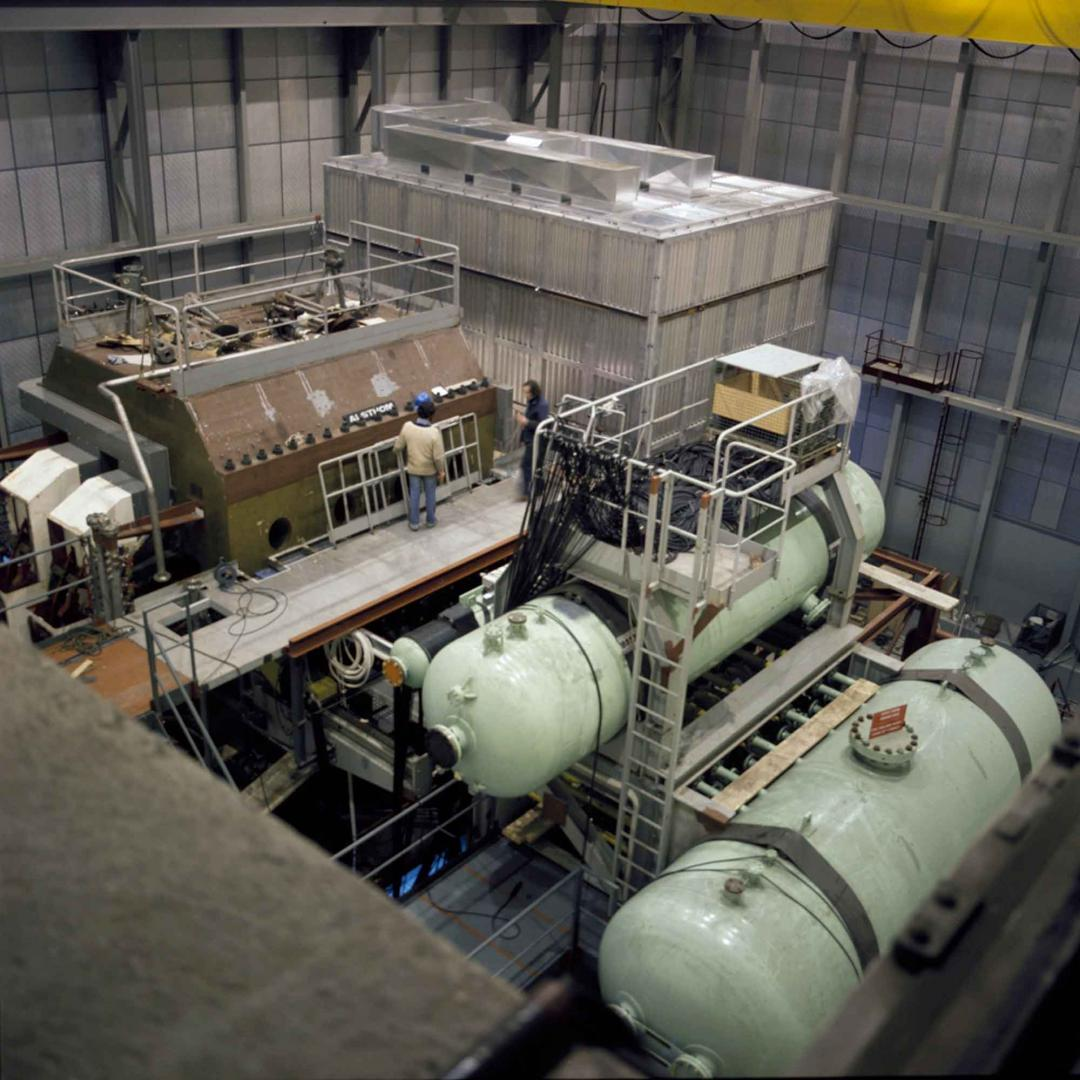
\includegraphics[width=\marginparwidth]{SM/gargamelle.jpg}
	\captionof{figure}{Gargamelle.}
	\label{GARGAMELLE}
}
\marginpar
{
	\centering
	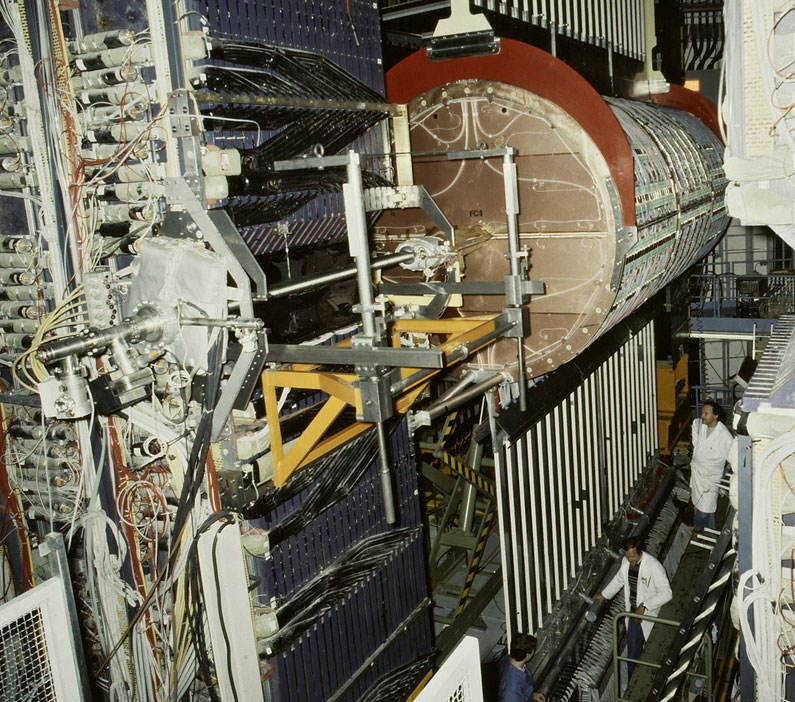
\includegraphics[width=\marginparwidth]{SM/ua1.jpg}
	\captionof{figure}{UA1.}
	\label{UA1}
}
\marginpar
{
	\centering
	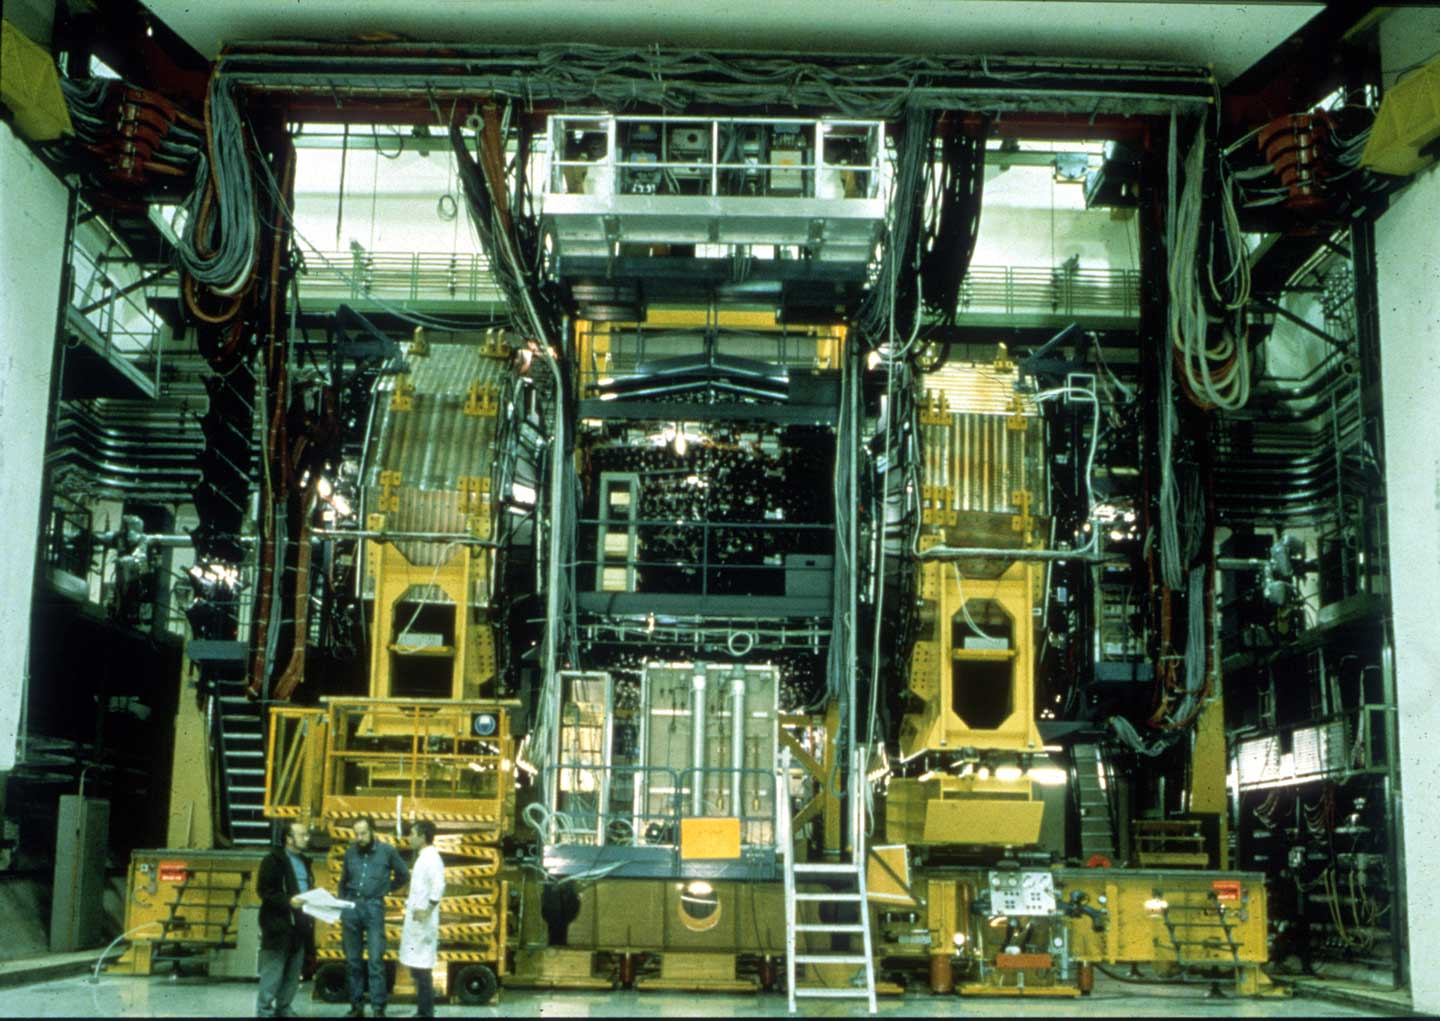
\includegraphics[width=\marginparwidth]{SM/ua2.jpg}
	\captionof{figure}{UA2.}
	\label{UA2}
}
\marginpar
{
	\centering
	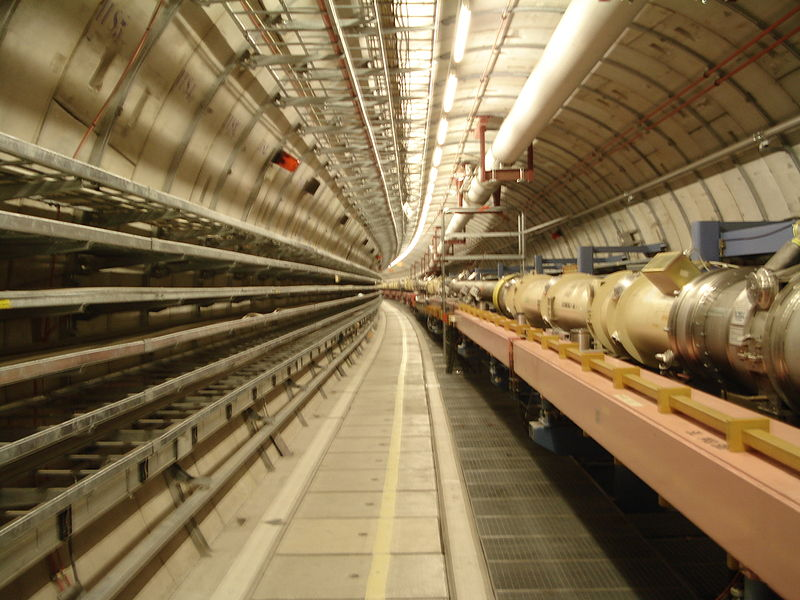
\includegraphics[width=\marginparwidth]{SM/HERA.jpg}
	\captionof{figure}{Tunnel du collisionneur HERA.}
	\label{HERA}
}
\marginpar
{
	\centering
	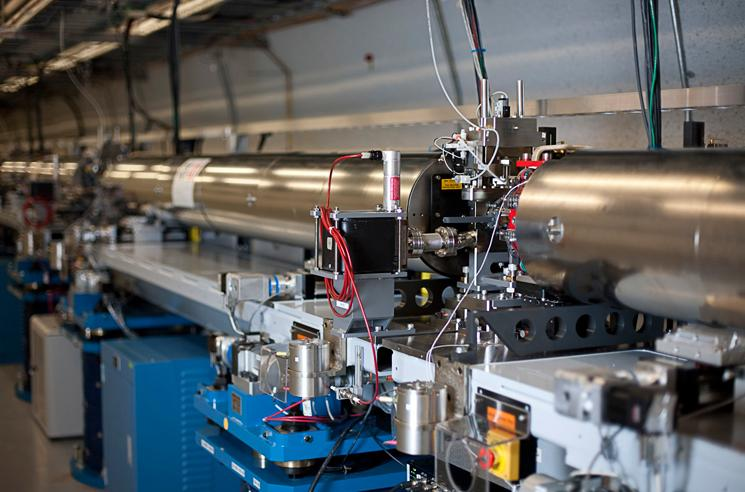
\includegraphics[width=\marginparwidth]{SM/slac.jpg}
	\captionof{figure}{Beam line du SLAC.}
	\label{SLAC}
}

De plus l'ensemble des mesures effectuées jusqu'à présent sont compatibles avec le Modèle Standard : La figure (cf.Fig~\ref{mesures}) montre la mesure de certains paramètres ainsi que leur "\textit{pull}" défini par :
\begin{equation}
\frac{O^{mesure}-O^{fit}}{\sigma^{mesure}}
\end{equation}
c'est-à-dire la déviation entre les mesures expérimentales et les prédictions théoriques en unités de l'incertitude expérimentale. Tous les \textit{pulls} sont inférieur à \num{3}$\sigma$. L'expérience et la théorie sont donc en très bon accord.

\begin{figure}[ht!]
\centering
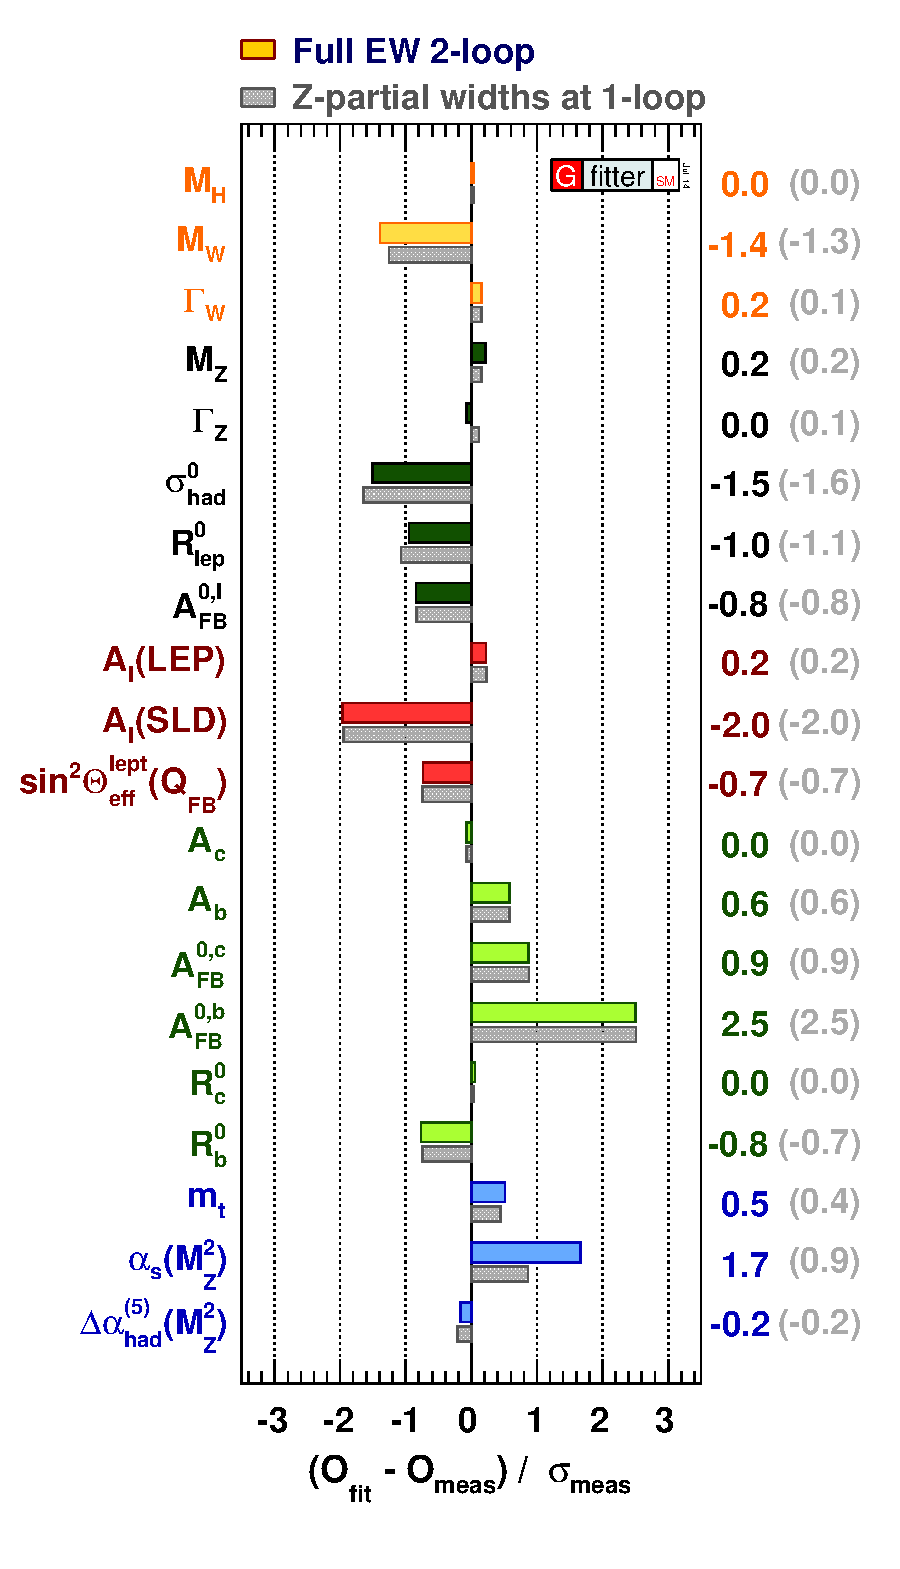
\includegraphics[width=0.50\textwidth]{SM/mesure.eps}
\captionof{figure}{Comparaison des résultats d'ajustement avec les mesures directes de certains paramètres du Modèle Standard.}
\label{mesures}
\end{figure}

\section{Les faiblesses du Modèle Standard}
\vspace*{-0.5cm}
Le Modèle Standard est en accord remarquable avec l'expérience. Cependant, plusieurs problèmes et questions non résolubles amènent à considérer le Modèle Standard comme une théorie effective, valable jusqu'à l'échelle du \si{\tera\eV}. Une nouvelle physique qui engloberait le Modèle Standard devrait apparaître à cette échelle d'énergie.

Parmi les principaux problèmes ou faits inexpliqués par le Modèle Standard, on peut citer :
\begin{itemize}[label=$\bullet$]
\item \textbf{Les neutrinos massifs :}
\marginpar
{
\centering
\includegraphics[width=\marginparwidth]{SM/kamiokande.jpg}
\captionof{figure}{Intérieur du détecteur Super-Kamiokande.}
\label{kamiokande}
}
\marginpar
{
\centering
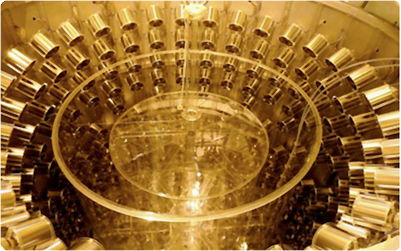
\includegraphics[width=\marginparwidth]{SM/chooz.jpg}
\captionof{figure}{Coeur du détecteur Double Chooz.}
\label{chooz}
} 
Les expériences Super-Kamiokande (cf.Fig~\ref{kamiokande}) et GALLEX portant sur l'observation du flux de neutrinos provenant du Soleil et les expériences Double Chooz (cf.Fig~\ref{chooz}) et K2K pour les flux de neutrinos de sources artificielles terrestres ont mis en évidence l'oscillation des neutrinos entre les saveurs leptoniques. Ces oscillations ne peuvent s'expliquer que si les neutrinos sont massifs et s'il existe des neutrinos droits. Bien que le Modèle Standard considère les neutrinos comme des particules de masse nulle et uniquement de parité gauche, il est facile d'y ajouter un neutrino droit dans chaque famille et les couplages au doublet \bsc{Higgs} correspondant afin de rendre compte de ces faits expérimentaux\footnote{C'est d'ailleurs cette extension du Modèle Standard qui est présentée dans ce chapitre.}. Cependant cela aggrave le problème de la hiérarchie des masses celles-ci s'étalant sur \num{10} ordres de grandeur !

\item \textbf{Le nombre de paramètres libres :} Le Modèle Standard contient \num{19} paramètres libres : les \num{3} constantes de couplage, les \num{2} paramètres $\lambda$ et $\mu^2$ du potentiel de \bsc{Higgs}, \num{9} couplages de \bsc{Yukawa}, les \num{3} angles, une phase pour les quarks dans la matrice CKM ainsi que l'angle associé au vide de QCD. Et d'autres encore en ajoutant le fait que les neutrinos soient massifs.

\item \textbf{Le nombre de familles :} Le nombre de familles a été expérimentalement obtenu en comparant la section efficace de production hadronique en fonction de l'énergie du centre de masse expérimentale $Z^{0}$ aux prédictions théoriques pour différents nombres de familles de neutrinos de masse négligeable. Actuellement on ne considère que trois familles (cf.Fig~\ref{neutrinos}). Cependant le fait que les neutrinos soient massifs permet l'existence de plus de trois familles à condition qu'ils aient une masse supérieure à $\frac{m_{Z^{0}}}{2}$.
\begin{figure}[ht!]
\centering
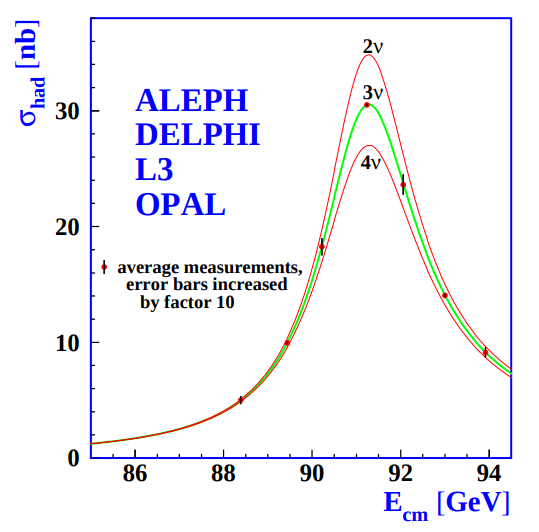
\includegraphics[width=0.48\textwidth]{SM/neutrinos.png}
\captionof{figure}{Mesures de la section efficace de production hadronique près de la résonance en $Z^0$. Les courbes indiquent les sections efficaces prédites pour deux, trois et quatre espéces de neutrinos de masses négligeables avec les couplages du Modèle Standard.}
\label{neutrinos}
\end{figure}

\item \textbf{La baryogénèse :} Le Modèle Standard est incapable d'expliquer l'asymétrie entre la quantité de baryons (matière) et d'anti-baryons (anti-matière) observée dans l'Univers.

\item \textbf{La gravitation :} Le Modèle Standard ne comporte pas l'interaction gravitationnelle. Aucune formulation quantique de la gravitation n'a encore été trouvée. La relativité générale, la meilleure théorie gravitationnelle, est malheureusement incompatible avec le Modèle Standard.

\item \textbf{Le problème de naturalité :} Il paraît naturel de considérer une échelle d'énergie ou le Modèle Standard cesse d'être valide. Or, les ordres supérieurs de la théorie perturbative ajoutent des corrections radiatives aux masses des différentes particules. En imposant une échelle d'énergie à la validité du Modèle Standard $\Lambda$, un "\textit{cut-off}", les corrections vont en dépendre. Pour le boson de \bsc{Higgs} et en considérant les diagrammes de la figure \ref{corrections} on peut écrire :
\begin{equation}
m_{h}^{2}=m_{0}^{2}-\delta m_{h}^{2}
\end{equation}
avec $m_{0}^{2}$ la masse "nue" du boson, $m_{h}^{2}$ la masse effective et $\delta m_{h}^{2}$ les corrections radiatives.

\begin{figure}[ht!]
\centering
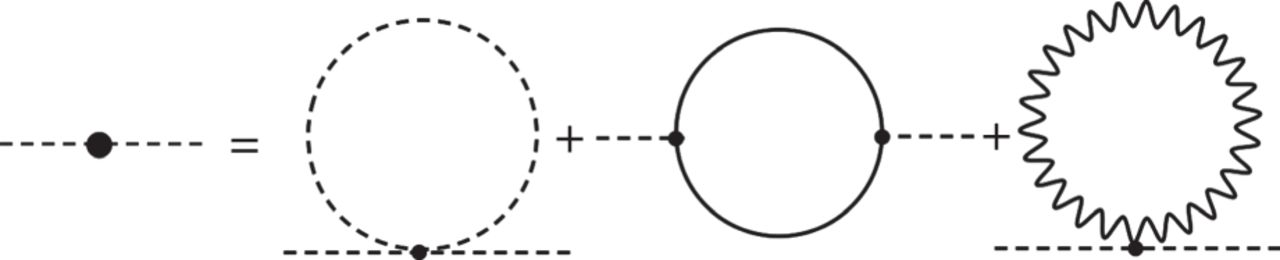
\includegraphics[width=0.35\textwidth]{SM/corrections.jpg}
\captionof{figure}{Corrections radiatives du premier ordre pour le boson de \bsc{Higgs}.}
\label{corrections}
\end{figure}

La contribution fermionique est de la forme :

\begin{equation}
\label{eq1}
\delta m_{h}^{2}=-\frac{y_{f}^{2}}{16\pi^{2}}\left(2\Lambda^{2}+6m_{f}\log\left(\frac{\Lambda}{m_{f}}\right)\cdots\right)
\end{equation}

En considérant un \textit{cut-off} de l'ordre de $\Lambda \sim$\SI{e16}{\giga\eV} il faut donc un accord à \num{e-30} entre $m_{0}^{2}$ et $\delta m_{h}^{2}$. Ce problème de hiérarchie et de réglage fin des paramètres ne semble pas naturel.

\item \textbf{La Matière Noire et l'Énergie Noire :} Des observations cosmologiques ont mis en évidence la présence de matière dite noire car elle n'émet pas et n'interagît pas avec les radiations électromagnétiques. Bien que n'ayant jamais été directement observée, son existence et certaines de ses propriétés peuvent être étudiées par leur effet gravitationnel sur le mouvement de la matière visible. Elle serait  également à l'origine de la formation des galaxies et des amas de galaxies, et de leur répartition de façon non uniforme dans l'Univers. D'après les observations du satellite Plank (cf.Fig~\ref{Plank}), la matière que nous connaissons ne compose que \num{4.9}\% du totale masse-énergie de l'Univers. La Matière Noire quant à elle ne compte que pour \num{26.8}\%. Les \num{68.3}\% restant sont composés d'Énergie Noire. Cette énergie serait responsable de l'accélération de l'expansion de l'Univers qui à été mise en évidence en \num{1998} par les projets \textit{Supernova Cosmology Project} et \textit{High-Z supernovae search team}. Ni la Matière Noire ni l'Énergie Noire ne sont décrites par le Modèle Standard.
\marginpar
{
\centering
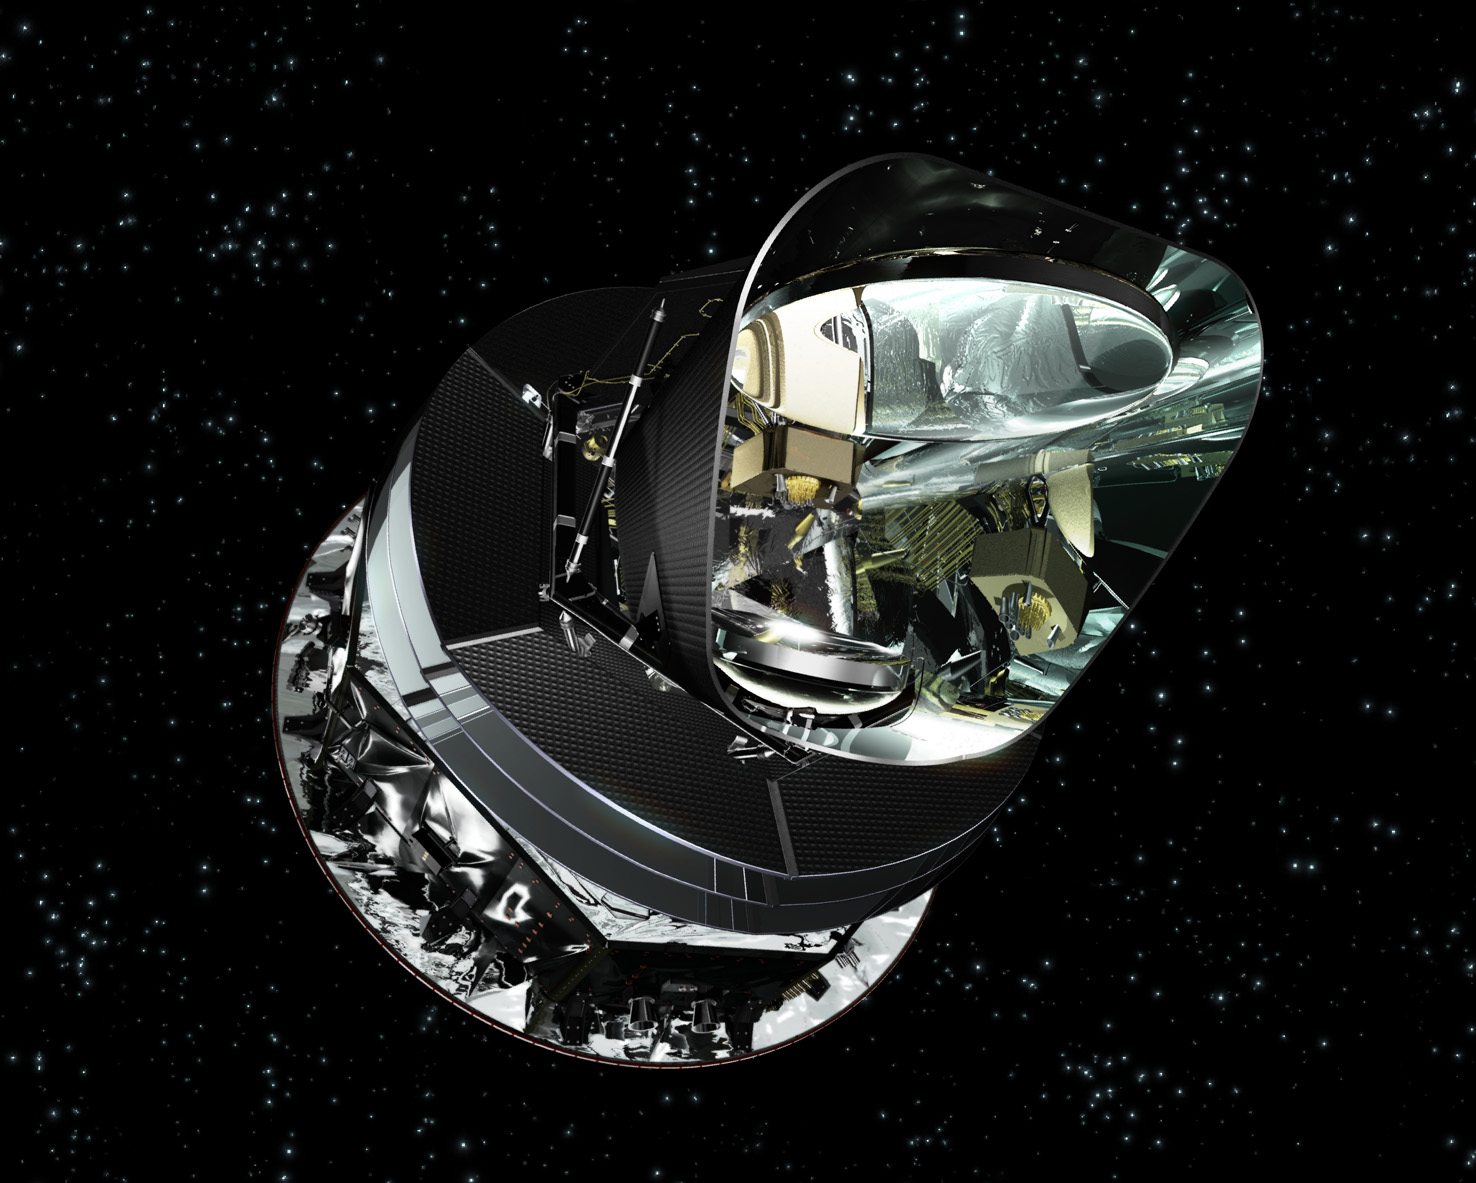
\includegraphics[width=\marginparwidth]{SM/plank.jpg}
\captionof{figure}{Le satellite \bsc{Plank}.}
\label{Plank}
} 

\item \textbf{La non unification des couplages : }Les constantes de couplage $\alpha_{1}$, $\alpha_{1}$ et $\alpha_{3}$ respectivement de l'interaction électromagnétique, faible et forte dépendent de l'échelle d'énergie. Il s'avère que ces trois constantes se rapprochent l'une de l'autre à haute énergie mais ne concourent pas en un seul point (cf.Fig~\ref{constantes}). Bien que n'étant pas en soit un problème, la convergence vers une valeur unique à haute énergie est nécessaire à une théorie "du tout" qui unifierait ces trois interactions. Le calcul de l'évolution de ces constantes par la méthode de renormalisation n'aboutissant pas à la convergence de ces trois constantes tend à prouver une lacune du Modèle Standard et son caractère effectif.
\begin{figure}[ht!]
\centering
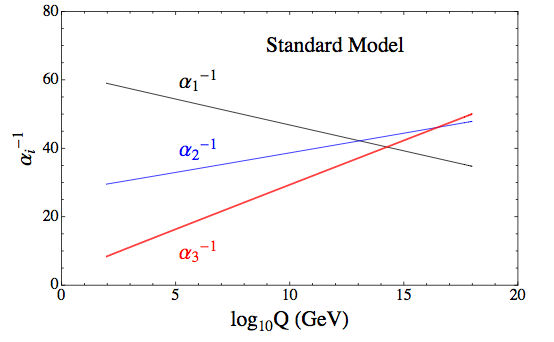
\includegraphics[width=0.50\textwidth]{SM/couplageSM.jpg}
\captionof{figure}{Évolution des constantes de couplage en fonction de l'échelle d'énergie dans le cas du Modèle Standard.}
\label{constantes}
\end{figure}
\end{itemize}

\section{Au delà du Modèle Standard}
Afin de résoudre certains de ces problèmes, de nombreux modèles théoriques ont été développés, cependant aucun d'entre eux n'est capable de répondre à toutes les questions et combler les lacunes du Modèle Standard. Certaines de ces théories sont des extensions de ce modèle, d'autres proposent des modèles complètement différents.

La majorité des modèles repose sur les symétries du Modèle Standard et cherche à les étendre; Soit en trouvant d'autres symétries internes (\textit{Grand Unified Theories} (GUT)), soit en liant les symétries internes et externes (supersymétrie (SUSY)) voire  modifier la nature même de l'espace-temps en ajoutant des dimensions supplémentaires par exemple.

\subsubsection{Les modèles de grande unification}
Ces modèles s'appuient sur le fait qu'il ait été possible de réunir dans le Modèle Standard trois des quatre interactions que nous connaissons et que leurs constantes de couplage se rapprochent l'une de l'autre à haute énergie. Il semble donc logique de vouloir unir ces trois interactions sous une même symétrie. Il n'existerait alors plus qu'un groupe $G$ et qu'une seule constante de couplage. Ces théories doivent bien sûr être renormalisables et leur groupe doit avoir comme sous-groupe celui du Modèle Standard $SU(3)\otimes SU(2) \otimes U(1)$. Les groupes $SU(5)$ et $SO(10)$ ont notamment été étudiés.

\subsubsection{Modèles à dimensions supplémentaires}
Ces modèles tentent de supprimer la naturalité et la hiérarchie des échelles d'énergie en faisant tendre l'échelle de \bsc{Planck} vers celle de l'interaction faible. Pour cela ils prennent comme hypothèse que l'espace-temps contient des dimensions supplémentaires enroulées compactes. L'interaction gravitationnelle évolue donc dans ces dimensions supplémentaires.

\subsubsection{La supersymétrie}
La supersymétrie a été introduite par \bsc{Weiss} et \bsc{Zumino} en \num{1974}. Elle consiste à supprimer les divergences quadratiques en les annulant grâce à l'ajout de termes supplémentaires. Pour cela on associe à chacun des fermions $f_{L}$ et $f_{R}$ un partenaire scalaire $\tilde{f}_{L}$ et $\tilde{f}_{R}$ possédant les mêmes nombres leptoniques et baryoniques. Ces partenaires contribuent donc aux diagrammes de corrections radiatives de la masse du \bsc{Higgs} (cf.Fig~\ref{corrections}). Les boucles scalaires ont une contribution positive contrairement aux boucles fermioniques, il est ainsi possible de supprimer le terme en $\Lambda^2$ de la formule \ref{eq1}. La masse du Higgs varie alors comme le logarithme de l'énergie $\Lambda$. On supprime ainsi le problème du \textit{fine-tuning} et de la naturalité. Les équations de renormalisation sont également modifiées et il est possible de faire concourir les constantes de couplage en un point. La supersymétrie est donc également un candidat à une théorie du "tout". La supersymétrie souffre cependant de certains problèmes, en effet, les particules superpartenaires sont censées être de même masse que les particules élémentaires. Or aucune superparticule n'a encore été détectée expérimentalement. Il faut donc introduire un mécanisme de brisure de la supersymétrie.

Nombre de ces théories postulent l'existence de nouvelles particules ou d'effets qui peuvent être vérifiés expérimentalement. Pour pouvoir savoir laquelle de ces théories décrit au mieux la nature ou contraindre ces modèles, il est nécessaire de construire de nouveaux accélérateurs toujours plus puissants et des détecteurs de plus en plus perfectionnés. 
